%    Copyright 2017 Marc Demierre, HES-SO//Master
%
% Licensed under the Apache License, Version 2.0 (the "License");
% you may not use this file except in compliance with the License.
% You may obtain a copy of the License at
%
% http://www.apache.org/licenses/LICENSE-2.0
%
% Unless required by applicable law or agreed to in writing, software
% distributed under the License is distributed on an "AS IS" BASIS,
% WITHOUT WARRANTIES OR CONDITIONS OF ANY KIND, either express or implied.
% See the License for the specific language governing permissions and
% limitations under the License.

% =============================================================================
% | HES-SO//Master - Thesis project report template                           |
% |                                                                           |
% | Originally based on the EPFL template, with many adjustements             |
% =============================================================================

% Document settings
\documentclass[a4paper,11pt,fleqn]{book}
\usepackage[utf8]{inputenc}
\usepackage[T1]{fontenc}
\usepackage[english,french]{babel}

% -----------------------------------------------------------------------------
% Preamble
% -----------------------------------------------------------------------------
% =============================================================================
% | Thesis metadata                                                           |
% =============================================================================

% Thesis info
\newcommand{\ThesisTitle}{LEVEE, IMPLEMENTATION DE « CONTROL- FLOW INTEGRITY » AU SEIN DE LLVM}
\newcommand{\ThesisSubject}{[ThesisSubject]}
\newcommand{\Orientation}{Technologies de l’information et de la communication (TIC)}
% \newcommand{\Keywords}{keyword1, keyword2, keyword3}
\newcommand{\Keywordsfr}{motclé1, motclé2, motclé3}

% Author
\newcommand{\AuthorFirstName}{Joël}
\newcommand{\AuthorLastName}{Gugger}
\newcommand{\AuthorEmail}{joel.gugger@master.hes-so.ch}
\newcommand{\Author}{\AuthorFirstName \ \AuthorLastName}

% Advisor
\newcommand{\AdvisorFirstName}{Pascal}
\newcommand{\AdvisorLastName}{Junod}
\newcommand{\AdvisorSchool}{[School]}
\newcommand{\AdvisorResearchUnit}{[ResearchUnit]}
\newcommand{\Advisor}{Prof. \AdvisorFirstName \ \AdvisorLastName}

% Main expert
\newcommand{\ExpertFirstName}{[FirstName]}
\newcommand{\ExpertLastName}{[LastName]}
\newcommand{\Expert}{\ExpertFirstName \ \ExpertLastName}
\newcommand{\ExpertLab}{[Lab/Company]}

% Dean
\newcommand{\Dean}{Prof. Fariba Moghaddam Bützberger}

% Place (for date and place)
\newcommand{\Date}{\today}
\newcommand{\Place}{Lausanne}
         % your project data
% ==================
% Template settings
% ==================

% General tools
% -------------
\usepackage{etoolbox}

% Page style
% ----------
\usepackage[margin=3cm, left=3.5cm, right=3.5cm, twoside=true]{geometry}
\usepackage{fancyhdr}
\setlength{\headheight}{14pt}
\renewcommand{\sectionmark}[1]{\markright{\thesection\ #1}}
\pagestyle{fancy}

% Standard pages (inside chapters)
\fancyhf{}
\renewcommand{\headrulewidth}{0.4pt}
\renewcommand{\footrulewidth}{0pt}
\fancyhead[OR]{\bfseries \nouppercase{\rightmark}}
\fancyhead[EL]{\bfseries \nouppercase{\leftmark}}
\fancyfoot[EL,OR]{\thepage}

% First page of chapters
\fancypagestyle{plain}{
	\fancyhf{}
	\renewcommand{\headrulewidth}{0pt}
	\renewcommand{\footrulewidth}{0pt}
	\fancyfoot[EL,OR]{\thepage}
}

% Imports for external PDFs
\fancypagestyle{addpagenumbersforpdfimports}{
	\fancyhead{}
	\renewcommand{\headrulewidth}{0pt}
	\fancyfoot{}
	\fancyfoot[RO,LE]{\thepage}
}

% Use empty style for page when clearing double pages
\def\cleartoodd{%
	\clearpage%
	\ifodd\value{page}\else\mbox{}\thispagestyle{empty}\newpage\fi%
}

\def\clearchap{%
	\ifodd\value{page}\else\mbox{}\thispagestyle{empty}\fi%
}

% \cleardoublepage replaced by \cleartoodd
\let\origdoublepage\cleardoublepage
\renewcommand{\cleardoublepage}{%
	\cleartoodd%
}

% Fonts
% -----

% Helvetica (Arial used in the MSE Word template)
\usepackage{helvet}

% Math
% ----
\usepackage{amsmath}  % better math

% Floats and figures
% ------------------
\usepackage{newfloat}          % floats
\usepackage[twoside]{caption}  % captions
\usepackage{subcaption}        % subcaptions
\usepackage[section]{placeins} % allows to put float barriers

% Float captions in italics, with label in margin
\DeclareCaptionLabelFormat{title}{#1 #2}
\DeclareCaptionLabelFormat{hangout}{\llap{#1 #2\hspace{5mm}}}
\captionsetup{
	format=hang,
	labelformat=hangout,
	singlelinecheck=false,
	font={it}
}

% Caption with source for figure
% TODO: improve this to use square brackets like the normal "caption"
\newcommand*{\captionsource}[3]{%
	\caption[{#1}]{%
		#2%

		\textbf{Source:} #3%
	}%
}

% Tables
% ------
\usepackage{booktabs} % much better tables
\usepackage{multirow} % allows to fuse rows
\usepackage{array}    % manipulate array
\usepackage{tabularx} % better tables

% Define new tabularx column types:
%  - R: streteched right aligned
%  - C: stretched centered
%  - N: left aligned, specified space
\newcolumntype{R}{>{\raggedleft\arraybackslash}X}%
\newcolumntype{C}{>{\centering\arraybackslash}X}%
\newcolumntype{N}[1]{>{\raggedleft\arraybackslash}p{#1}}

% Set row height multiplicator to provide more breathing space
\renewcommand{\arraystretch}{1.3}

% Bibliography
% -------------------

% Use biber, with numeric style and no sorting (citation order)
\usepackage[
backend=biber,
style=numeric,
sorting=none,
bibencoding=auto
]{biblatex}
\addbibresource{03-tail/bibliography.bib}


% Tables of contents, figures, tables and listings
% ------------------------------------------------
\usepackage{tocloft}
\newlistof{listing}{lol}{Liste des codes sources}
\setcounter{tocdepth}{1} % Depth to 'section'
\setlength{\cftfigindent}{0pt}  % remove indentation from figures in lof
\setlength{\cftfignumwidth}{1cm}
\setlength{\cfttabindent}{0pt}  % remove indentation from tables in lot
\setlength{\cfttabnumwidth}{1cm}
\setlength{\cftlistingindent}{0pt}
\setlength{\cftlistingnumwidth}{1cm}

% Mini tables of contents
% -----------------------
\usepackage{minitoc}

% no "Contents" title
\mtcsettitle{minitoc}{Contenu du chapitre}

% Layout
\setlength{\mtcindent}{-0.5em}
\mtcsetoffset{minitoc}{-1em}

% Spacing above and below table
\mtcsetfeature{minitoc}{before}{\vspace{0.5cm}}
\mtcsetfeature{minitoc}{after}{\vspace{0.5cm}}
% \renewcommand{\mtifont}{\sffamily\bfseries\large}
% \renewcommand{\mltfont}{\small\rmfamily}

% Colors & graphics
% -----------------
\usepackage[table]{xcolor}    % colors
\usepackage[pdftex]{graphicx} % graphics importing
\graphicspath{{02-main/figures/}}
\definecolor{gray80}{gray}{0.80}


% Code and syntax highlighting
% ----------------------------
\usepackage[newfloat]{minted}   % code highlighting

% Typography
% ----------
\usepackage{csquotes}                    % paragraph indentation and spacing
\usepackage[defaultlines=3,all]{nowidow} % avoid widows and orphans
\usepackage{microtype}                   % typographic improvements
% \usepackage{parskip}                     % No indent and auto-space between paragraphs
\usepackage[super]{nth}

\usepackage{paralist}
\usepackage{enumitem}
\setlist{after=\vspace{\baselineskip}}

% Section and chapters headings
% -----------------------------
\usepackage[explicit]{titlesec} % titles formatting
%\usepackage{titletoc} % titles formatting in ToC etc
%\usepackage{sectsty}  % sectioning commands

% -- Chapters --
% Remove "Chapter N" and use a sans-serif font

% Set layout lengths
\setlength{\headheight}{8mm}
\setlength{\footskip}{1.5cm}
\addtolength{\textheight}{-.5cm}

\titlespacing{\chapter}{-5mm}{-10mm}{3mm}
\titlespacing{\section}{-5mm}{3mm}{3mm}
\titlespacing{\subsection}{-5mm}{3mm}{2mm}
\titlespacing{\subsubsection}{-5mm}{2mm}{3mm}


%\titleformat{\chapter}[block]
%{\Huge}
%{\thechapter\hspace{12pt}\textcolor{gray80}{|}\hspace{12pt}}
%{0pt}
%{\Huge\bfseries}

\titleformat{\chapter}{\Huge\bfseries}{\llap{\thechapter\hspace{12pt}\textcolor{gray80}{|}}}{0mm}{%
	\hfill\begin{minipage}[t]{\dimexpr\textwidth}\raggedright#1\end{minipage}%
}
\titleformat{\section}{\Large\bfseries}{\llap{\thesection}}{0mm}{%
	\hfill\begin{minipage}[t]{\dimexpr\textwidth}\raggedright#1\end{minipage}%
}
\titleformat{\subsection}{\large \bfseries}{\llap{\thesubsection}}{0mm}{%
	\hfill\begin{minipage}[t]{\dimexpr\textwidth}\raggedright#1\end{minipage}%
}
\titleformat{\subsubsection}{\bfseries}{\llap{\thesubsubsection}}{0mm}{%
	\hfill\begin{minipage}[t]{\dimexpr\textwidth}\raggedright#1\end{minipage}%
}

% Misc
% ------
\usepackage{lipsum}    % filler text
\usepackage{blindtext} % random text
\usepackage{lscape}    % easy landscape pages
\usepackage{pdflscape} % landscape pages for PDFs

% Allow email typesetting
\newcommand{\email}[1]{%
	\href{mailto:#1}{\textit{#1}}%
}

% References
% -----------
\usepackage{url}
\makeatletter
\g@addto@macro{\UrlBreaks}{\UrlOrds}
\makeatother

% pdf metadata
\usepackage[
	pdfauthor={\Author},
	pdftitle={\ThesisTitle},
	pdfsubject={\ThesisSubject},
	pdfkeywords={\Keywordsfr}
	pdfduplex=DuplexFlipLongEdge]{hyperref}

% Hyperlinks
\hypersetup{
	colorlinks=true,
	linkcolor=black,
	citecolor=black,
	filecolor=black,
	urlcolor=black,
}
\providecommand*{\listingautorefname}{Listing}


% Glossary
% --------
\usepackage[xindy,toc]{glossaries}
% Terms
% -----
% format:  \newglossaryentry{<label>}{<settings>}
% example: \newglossaryentry{computer}
%{
%	name=computer,
%	description={is a programmable machine that receives input,
%		stores and manipulates data, and provides
%		output in a useful format}
%}

% \newglossaryentry{nosql}
% {
% 	name=NoSQL,
% 	description={Database not using the relational model and the \acrshort{sql} language}
% }


% Display ASLR
\newglossaryentry{aslr}
{
	name=ASLR,
	description={Address Space Layout Randomization, technique permettant de rendre aléatoire la position des ségments mémoires}
}

\newglossaryentry{cg-cfi}
{
	name=Coarse-grained CFI,
	description={Coarse-grained CFI est une implémentation simplifiée du principe de Control-Flow integrity, échangeant sécurité contre plus de performances}
}

\newglossaryentry{fg-cfi}
{
	name=Finest-grained CFI,
	description={Finest-grained CFI est une implémentation plus complète du principe de Control-Flow integrity. Garantissant une bonne sécurité mais ayant un coût élevé en performances}
}

\newglossaryentry{dep}
{
	name=DEP,
	description={Data Execution Prevention, technique permettant de marquer un espace vituel de mémoire non-exécutable}
}

\newglossaryentry{nx}
{
	name=NX,
	description={NX bit pour No-eXecute bit est une technique utilisée dans les processeurs pour dissocier les zones de mémoire contenant des instructions des zones contenant des données}
}

\newglossaryentry{stackCookies}
{
	name={Stack cookies},
	description={Les stack cookies, ou stack canaries, sont des valeurs déposées sur la pile d'exécution après la valeur de retour lors de l'appel d'une fonction et son controlées à l'épilogue de la-dite fonction}
}

\newglossaryentry{stackCanaries}
{
	name={Stack canaries},
	description={Les stack canaries sont un synonyme de stack cookies}
}

\newglossaryentry{levee}
{
	name={Levee},
	description={Levee est une implémentation des concepts de protection CPI, CPS et Safe Stack. Actuellement, mai 2017, une partie du projet a été intégré au sein de LLVM sous le nom de Safe Stack}
}

\newglossaryentry{llvm}
{
	name={LLVM},
	description={LLVM, à la base Low Level Virtual Machine et maintenant nom à part entière, est une approche divergente aux compilateur tel que GCC et une collection d'outils de compilation}
}


% Acronyms
% --------
% format:  \newacronym{<label>}{<abbrv>}{<full>}
% example: \newacronym{lvm}{LVM}{Logical Volume Manager}
% plural:  \newacronym[longplural={Frames per Second}]{fpsLabel}{FPS}{Frame per Second}

% % Display Address Space Layout Randomization (ASLR)
% \newacronym{aslr}{ASLR}{Address Space Layout Randomization}


\newacronym{epfl}{EPFL}{École polytechnique fédérale de Lausanne}
\newacronym{nop}{NOP}{No Operation}
\newacronym{cfg}{CFG}{Control-Flow graph}
\newacronym{cfi}{CFI}{Control-Flow integrity}
\newacronym{eof}{EOF}{End Of File}
\newacronym{rop}{ROP}{Return Oriented Programming}
\newacronym{cpi}{CPI}{Code-pointer integrity}
\newacronym{cps}{CPS}{Code-pointer separation}

% \newacronym{api}{API}{Application Programming Interface}
%
% \newacronym{cep}{CEP}{Complex Event Processing}
% \newacronym{ci}{CI}{Continuous Integration}
% \newacronym{cqrs}{CQRS}{Command Query Responsibility Segregation}
% \newacronym{crud}{CRUD}{Create-Read-Update-Delete}
%
% \newacronym{dag}{DAG}{Directed Acyclic Graph}
% \newacronym{dsl}{DSL}{Domain Specific Language}
%
% \newacronym{eca}{ECA}{Event Condition Action}
% \newacronym{elk}{ELK}{Elasticseach Logstash and Kibana}
% \newacronym{efk}{EFK}{Elasticseach Fluentd and Kibana}
% \newacronym{epa}{EPA}{Event Processing Agent}
% \newacronym{epn}{EPN}{Event Processing Network}
%
% \newacronym{gelf}{GELF}{Graylog Extended Log Format}
% \newacronym{ge}{GE}{Generic Enabler}
%
% \newacronym{ide}{IDE}{Integrated Development Environment}
% \newacronym{iot}{IoT}{Internet of Things}
%
% \newacronym{jar}{JAR}{Java ARchive}
% \newacronym{jmx}{JMX}{Java Management Extensions}
% \newacronym{json}{JSON}{JavaScript Object Notation}
% \newacronym{jvm}{JVM}{Java Virtual Machine}
%
% \newacronym{poc}{PoC}{Proof of Concept}
%
% \newacronym{rest}{REST}{Representational state transfer}
% \newacronym{rest_markup}{reST}{reStructuredText}
% \newacronym{rpc}{RPC}{Remote Procedure Call}
%
% \newacronym{sql}{SQL}{Structured  Query Language}
%
% \newacronym{uuid}{UUID}{Universally Unique Identifier}
% \newacronym{uri}{URI}{Universal Resource Identifier}

\makeglossaries
    % template settings
% ===========================================
% = Codestyles for minted syntax highlighting
% ===========================================


% How to use (replace 'java' with language name):
% - code blocks:
%     \begin{javacode}
%     CODE
%     \end{javacode}
% - files:
%     full: \javafile{PATH}
%     extract: \javafile[startline=x, endline=y]{PATH}

\usemintedstyle{trac}
\definecolor{mintedBg}{rgb}{0,0,0}

% C
\newminted{c}{
	% frame=single,
	% framesep=6pt,
	breaklines=true,
	fontsize=\scriptsize,
	linenos,
	% bgcolor=mintedBg
}
\newmintedfile{c}{
	% frame=single,
	% framesep=6pt,
	breaklines=true,
	fontsize=\scriptsize,
	linenos,
	% bgcolor=mintedBg
}
% Python
\newminted{python}{
	% frame=single,
	% framesep=6pt,
	breaklines=true,
	fontsize=\scriptsize,
	linenos,
	% bgcolor=mintedBg
}
\newmintedfile{python}{
	% frame=single,
	% framesep=6pt,
	breaklines=true,
	fontsize=\scriptsize,
	linenos,
	% bgcolor=mintedBg
}

\newmintedfile{docker}{
	% frame=single,
	% framesep=6pt,
	breaklines=true,
	fontsize=\scriptsize,
	linenos,
	% bgcolor=mintedBg
}

% % Java
% \newminted{java}{frame=single, framesep=6pt, breaklines=true, fontsize=\scriptsize}
% \newmintedfile{java}{frame=single, framesep=6pt, breaklines=true,
% fontsize=\scriptsize}
%
% % Scala
% \newminted{scala}{frame=single, framesep=6pt, breaklines=true, fontsize=\scriptsize}
% \newmintedfile{scala}{frame=single, framesep=6pt, breaklines=true,
% 	fontsize=\scriptsize}
%
% % Clojure
% \newminted{clojure}{frame=single, framesep=6pt, breaklines=true, fontsize=\scriptsize}
% \newmintedfile{clojure}{frame=single, framesep=6pt, breaklines=true,
% 	fontsize=\scriptsize}
%
% % Python
% \newminted{python}{frame=single, framesep=6pt, breaklines=true, fontsize=\scriptsize}
% \newmintedfile{python}{frame=single, framesep=6pt, breaklines=true, fontsize=\scriptsize}
%
% % Sql
% \newminted{sql}{frame=single, framesep=6pt, breaklines=true, fontsize=\scriptsize}
% \newmintedfile{sql}{frame=single, framesep=6pt, breaklines=true, fontsize=\scriptsize}
%
% % Json
% \newminted{json}{frame=single, framesep=6pt, breaklines=true, fontsize=\scriptsize}
% \newmintedfile{json}{frame=single, framesep=6pt, breaklines=true,
% 	fontsize=\scriptsize}
%
% % Yaml
% \newminted{yaml}{frame=single, framesep=6pt, breaklines=true,
% fontsize=\scriptsize}
% \newmintedfile{yaml}{frame=single, framesep=6pt, breaklines=true,
% 	fontsize=\scriptsize}
%
% % Plain text
% \newminted{text}{frame=single, framesep=6pt, breaklines=true, breakanywhere, fontsize=\scriptsize}
% \newmintedfile{text}{frame=single, framesep=6pt, breaklines=true, breakanywhere, fontsize=\scriptsize}
       % code styles for minted
% ========================
% = Custom Settings
% ========================

\setlength{\parindent}{15pt}
\setlength{\parskip}{0.0pt plus 1.0pt}


% \providecommand*{\listingautorefname}{Listing}
% \renewcommand{\lstlistingname}{Code}% Listing -> Algorithm
\def\lstlistingautorefname{Alg.}

% Create a new environment for breaking code listings across pages.
\newenvironment{longlisting}{\captionsetup{type=listing}}{}

\usepackage{pdfpages}
\usepackage{emptypage}
\usepackage{amsfonts}
\usepackage{dirtytalk}
\usepackage{mathtools}
\usepackage{nccmath}
\usepackage{tabularx}
\usepackage{hhline}

\newtheorem{theorem}{Theorem}[section]
\newtheorem{definition}{Definition}[section]
\newtheorem{lemma}[theorem]{Lemma}
\newtheorem{postulate}[theorem]{Postulate}
  % your custom packages etc

\begin{document}
% -----------------------------------------------------------------------------
% Front matter
% -----------------------------------------------------------------------------
\frontmatter

\dominitoc

% ==========================================================================
% = HES-SO Master thesis title page (modeled after Word template, 2016-2017)
% ==========================================================================

\begin{titlepage}
\newgeometry{margin=2.5cm}
{\fontfamily{phv}\fontseries{mc}\selectfont
	\begin{flushright}
		\begin{minipage}{0.5\textwidth}
			\begin{flushleft}
				\includegraphics[width=0.9\textwidth]{img/mse_logo}
			\end{flushleft}
		\end{minipage}%
		\begin{minipage}{0.5\textwidth}
			\begin{flushright}
				\includegraphics[width=0.6\textwidth]{img/hesso_logo}
			\end{flushright}
		\end{minipage}
		\begin{flushleft}
			\footnotesize
			Master of Science HES-SO in Engineering \\
			Av. de Provence 6 \\
			CH-1007 Lausanne
		\end{flushleft}
		~\\[0.5cm]

		{
		\Huge Master of Science HES-SO in Engineering\\[0.5cm]
		}

		{
		\LARGE Orientation: \Orientation\\[0.5cm]
		~\\[1cm]
		}
		% Title
		{
			\Huge
			\ThesisTitle \\[1.5cm]
		}
		{
			\large
			Fait par\\[-0.3cm]
			\Huge \Author \\[0.8cm]
		}
		{
			\large
			Sous la direction de \\
			\Advisor \\
			\AdvisorResearchUnit \\[0.5cm]
		}
		{
			\large
			Expert externe
			\Expert \\
			\ExpertLab
		}
		\vfill

		% Bottom of the page
		{\large \Place, HES-SO//Master, le \Date}

	\end{flushright}
}
\restoregeometry
\end{titlepage}


% Page for student info and signatures
\cleardoublepage
\setlength{\parindent}{0pt}

\chapter*{Information about this report}

\vspace{\fill}

\textbf{Contact information}

\begin{tabularx}{\textwidth}{N{2.5cm}X}
	Author:	 & \AuthorFirstName \AuthorLastName \\
	& MSE Student \\
	& HES-SO//Master \\
	& Switzerland \\
	Email: & \email{\AuthorEmail}
\end{tabularx}

\vspace{\fill}

\textbf{Declaration of honor}

{\renewcommand{\arraystretch}{2}
\begin{tabularx}{\textwidth}{N{2.5cm}X}
	& I, undersigned, \Author, hereby declare that the work submitted is
	the result of a personal work. I certify that I have not resorted to
	plagiarism or other forms of fraud. All sources of information used and the
	author quotes were clearly mentioned. \\
	Place, date: & \underline{\hspace{7cm}} \\
	Signature: & \underline{\hspace{7cm}}
\end{tabularx}
}

\vspace{\fill}

\textbf{Validation}

Accepted by the HES-SO//Master (Switzerland, Lausanne) on a proposal from:

\vspace{0.5cm}

\Advisor, Thesis project advisor

\Expert, \ExpertLab, Main expert

\vspace{1cm}

Place, date: \underline{\hspace{8cm}}

\vspace{3cm}

{ \renewcommand{\arraystretch}{1.5}
\begin{tabularx}{\textwidth}{X X}
	\Advisor  & \Dean\\
	Advisor   & Dean, HES-SO//Master\\
\end{tabularx}
}

% \setlength{\parindent}{0pt}
%
% \chapter*{À propos du rapport}
%
% \vspace{\fill}
%
% \textbf{Information de contact}
%
% \begin{tabularx}{\textwidth}{N{2.5cm}X}
% 	Auteur :	 & \AuthorFirstName \ \AuthorLastName \\
% 	& Étudiant MSE \\
% 	& HES-SO//Master \\
% 	& Suisse \\
% 	Email : & \email{\AuthorEmail}
% \end{tabularx}
%
% \vspace{\fill}
%
% \textbf{Déclaration d'honeur}
%
% {\renewcommand{\arraystretch}{2}
% \begin{tabularx}{\textwidth}{N{2.5cm}X}
% 	& Je, soussigné, \Author, déclare que ce travail fourni est le résultat d'un travail personnel. Je certifie n'avoir usé d'aucun plagiat ou autres formes de fraudes. Toutes les ressources utilisées ainsi que les auteurs des citations ont été distinctement mentionées. \\
%
% 	% & I, undersigned, \Author, hereby declare that the work submitted is
% 	% the result of a personal work. I certify that I have not resorted to
% 	% plagiarism or other forms of fraud. All sources of information used and the
% 	% author quotes were clearly mentioned. \\
% 	Lieu, date: & \underline{\hspace{7cm}} \\
% 	Signature: & \underline{\hspace{7cm}}
% \end{tabularx}
% }
%
% \vspace{\fill}
%
% \textbf{Validation}
%
% Accepté par la HES-SO//Master (Suisse, Lausanne) sur proposition de :
%
% \vspace{0.5cm}
%
% \Advisor, conseiller du projet d’approfondissement
%
% \Expert, \ExpertLab, expert
%
% \vspace{1cm}
%
% Lieu, date: \underline{\hspace{8cm}}
%
% \vspace{3cm}
%
% { \renewcommand{\arraystretch}{1.5}
% \begin{tabularx}{\textwidth}{X X}
% 	\Advisor  & \Dean\\
% 	Conseiller   & Resp. de la filière HES-SO//Master\\
% \end{tabularx}
% }
%
% \setlength{\parindent}{15pt}


% Acknowledgments (your dedication etc)
\cleardoublepage
\chapter*{Remerciements}
\markboth{Remerciements}{Remerciements}
\addcontentsline{toc}{chapter}{Remerciements}

% -- Your text goes here --
\lipsum[1-2]


% % Preface (to be written by someone else)
% \cleardoublepage
% % \chapter*{Preface}
% \markboth{Preface}{Preface}
% \addcontentsline{toc}{chapter}{Preface}
% % put your text here
% A preface is not mandatory. It would typically be written by some other person (eg your thesis director).
%
% \lipsum[1-2]
%
% \bigskip
%
% \noindent\textit{Lausanne, 12 Mars 2011}
% \hfill T.~D.


% French + English abstracts
\cleardoublepage
% English abstract
\chapter*{Abstract}
\addcontentsline{toc}{chapter}{Abstract} % adds an entry to the table of contents

Bitcoin is a decentralized peer-to-peer currency that allow users to to pay for
things electronically. Bitcoin was created by a pseudonymous software developer
going by the name of Satoshi Nakamoto in 2008, as an electronic payment system
based on mathematical proof. Yet the largest challenge in Bitcoin for the coming
years is scalability. Currently, Bitcoin can only handle a few transactions per
second on the network. This is not sufficient in comparison to large payment
infrastructures, which allow tens of thousands of transactions per second. As a
potential scalability solution, the idea of payment channels was suggested by
Satoshi in an email to Mike Hearn. A one-way payment channel specific for retail
commercial transactions is presented, analyzed and optimized with threshold
cryptography. The threshold scheme selected has been adapted and implemented
into the Bitcon cryptographic library to compute a special two-party threshold
ECDSA signature.

\vskip0.5cm
\noindent\textbf{Keywords:}
\Keywords

% (\url{https://en.bitcoin.it/wiki/Payment_channels#Nakamoto_high-frequency_transactions};
% \url{https://lists.linuxfoundation.org/pipermail/bitcoin-dev/2013-April/002417.html})


% Table of contents
\cleardoublepage
\phantomsection
% \addcontentsline{toc}{chapter}{Contents}
\tableofcontents

% List of figures
\cleardoublepage
\phantomsection
\addcontentsline{toc}{chapter}{Table des figures}
\listoffigures

% List of tables
\cleardoublepage
\phantomsection
\addcontentsline{toc}{chapter}{Liste des tableaux}
\listoftables

% List of listings
\cleardoublepage
\phantomsection
\addcontentsline{toc}{chapter}{Liste des codes sources}
\listoflistings

% Restore paragraphs
\setlength{\parskip}{1em}

% Bold fonts for sections in minitoc
\renewcommand{\cftsecfont}{\sffamily\bfseries}
\renewcommand{\cftsecleader}{\sffamily\bfseries\cftdotfill{\cftdotsep}}
\renewcommand{\cftsecpagefont}{\sffamily\bfseries}


% -----------------------------------------------------------------------------
% Main matter
% -----------------------------------------------------------------------------
\mainmatter

\setlength{\parindent}{15pt}
\setlength{\parskip}{0.0pt plus 1.0pt}

% Chapters
\setcounter{mtc}{5} % Help minitoc skip the front matter chapters
\chapter{Introduction}
\label{chap:introduction}

Bitcoin is a decentralized peer-to-peer currency that allows users to pay for
things electronically. Thousands of other cryptocurrencies exist, but only some
of them are really interesting from a political, economical or technical point
of view. Bitcoin was created by a pseudonymous software developer going by the
name of Satoshi Nakamoto in 2008, as an electronic payment system based on
mathematical proof. The idea was to produce a means of exchange, independent of
any central authority and censorship-resistant, which could be transferred
electronically in a secure, verifiable and immutable way. The blockchain is the
output of this secure, verifiable and immutable mathematical proof.

The most significant challenge in Bitcoin for the coming years is scalability.
Currently, Bitcoin enforces a block-size limit which is equivalent to only a few
transactions per second on the network. This amount is not sufficient in
comparison to large payment infrastructures, which allow tens of thousands of
transactions per second and even more at peak times such as Christmas.  To
address this there are some proposals to modify the transaction structure (SegWit \cite{SegWitBIP}),
some to modify the block-size limit (SegWit2x) and others to
create a second layer on top of the Bitcoin protocol (Lightning Network \cite{poon2016bitcoin}).
In the same idea of a second layer, this thesis explores the
implementation of a unidirectional payment channel for retail commercial
transactions that allows two parties to
transact with cryptocurrencies while minimizing the number of transactions needed
on the blockchain in a secure and trustless way. Every type of payment channel needs
multi-signature addresses to secure the funds. A cryptographic threshold scheme
might improve these schemes significantly. Finding such a threshold scheme that
fulfills the requirements is not trivial. The threshold scheme selected for this work is
adapted to the needs of channels, and is implemented in the Bitcoin cryptographic
library to compute a particular two-party threshold ECDSA signature.

\chapter{Historique des mécanismes de protection}
\label{chap:historique}

La gestion de la mémoire est un des composants le plus complexe d'un système d'exploitation moderne, ce qui rend le sujet bien plus vaste que ce que l'on peut traiter dans ce rapport. Cependant, il m'a été nécessaire de parcourir les principaux concepts pour pouvoir en comprendre les enjeux.

Dans ce chapitre, un bref récapitulatif de cette gestion est fait en préambule de la partie historique des attaques et des mécanismes de protection. Les cas expliqués dans ce rapport sont volontairement simplifiés de manière à comprendre l'aspect conceptuel et non la mise en pratique dans un environement réel. Exploiter dans un environement réel certaines des attaques brièvement décrites par la suite peut occuper le volume d'un rapport au moins égal à celui-ci.

La description du fonctionnement de la mémoire est inspirée d'articles tirés du blog de Gustavo Duarte \cite{AnatomyOfAProgramInMemory, HowTheKernelManagesYourMemory, JourneyToTheStackPartI}. À des fins de simplicité, les concepts exposés sont basé sur une architecture 32~bits. Dans le cas de changements notables entre architectures, un complément spécifique à l'architecture 64~bits est donné. Les termes anglais sont mentionnés une première fois lors de leurs traductions, le document utilise ensuite la traduction française.

\minitoc

\newpage

% ---------------------------------------------------------------------------
\section{Rappel sur la gestion de la mémoire}

La mémoire d'un programe est gérée selon un schéma bien défini. Chaque processus du système d'exploitation voit sa mémoire définie dans un espace virtuel \og virtual address space \fg, l'isolant complètement du reste des processus. Ce espace est égal à 4~Go dans un système 32~bits. Dans le cas d'une architecture 64~bits, l'espace disponible n'utilise pas $2^{64}$ octets (16~Eo), mais uniquement les 48~bits les moins significatifs, et donc $2^{48}$ octets (256~To) \cite{64bitComputing,VirtualAddressSpaceDetails}. Le système d'exploitation est ensuite responsable de faire le lien entre cet espace virtuel et l'espace d'adressage physique.

\subsection{Segmentation}

La mémoire virtuelle est scindée en deux parties principales. La première, ayant les adresses mémoires allant de \mintinline{c}{0xc0000000} à \mintinline{c}{0xffffffff} (en 32 bits), est reservée, sous Linux, au noyau du système d'exploitation. La seconde, quant à elle, correspond à l'espace disponible du processus courant.

\begin{figure}[H]
	\centering
	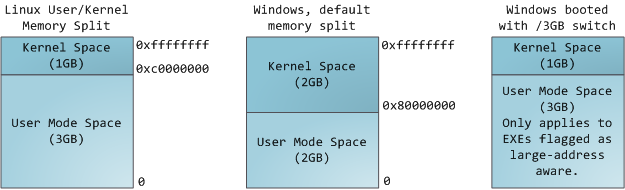
\includegraphics[width=0.8\columnwidth]{kernelUserMemorySplit}
	\captionsource{Répartition de l'espace mémoire du kernel}
	{Répartition de l'espace mémoire virtuel entre le noyau et le programme, par G.~Duarte}
	{\url{http://duartes.org/gustavo/blog/post/anatomy-of-a-program-in-memory/}}
	\label{fig:kernelUserMemorySplit}
\end{figure}

L'espace réservé au processus est ensuite découpé en différents segments tel que la pile \og stack \fg ou le tas \og heap \fg. Ces segments sont des plages mémoires continues gérées par le système d'exploitation. Dans le cas d'un processus Linux, les segments sont répartis ainsi :

\begin{figure}[H]
	\centering
	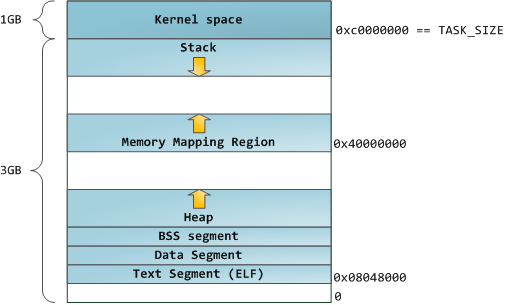
\includegraphics[width=.7\columnwidth]{linuxClassicAddressSpaceLayout}
	\captionsource{Segmentation de la mémoire d'un processus Linux 32 bits}
	{Segmentation de la mémoire d'un processus Linux en 32 bits, par G.~Duarte}
	{\url{http://duartes.org/gustavo/blog/post/anatomy-of-a-program-in-memory/}}
	\label{fig:linuxClassicAddressSpaceLayout}
\end{figure}

\vfill

La pile d'exécution permet de gérer le flot de contrôle de l'application. À chaque appel de fonction, une nouvelle structure de pile \og stack frame \fg est ajoutée à la pile, puis est retirée lorsque la fonction se termine. La pile d'exécution grandit vers le bas, c'est-à-dire que les adresses mémoires décroissent lorsque la pile se remplit. Il est possible que la pile veuille s'étendre au-delà de sa taille maximum, c'est le cas du dépassement de pile \og stack overflow \fg. Dans ce cas, le programme reçoit une erreur de segmentation, \og segmentation fault \fg en anglais, et s'arrête.

Le segment \og memory mapping region \fg permet au noyau de copier en mémoire le contenu de certains fichiers de manière à augmenter les performances. Ce segment est généralement utilisé pour charger les bilbiothèques dynamiques. Il peut aussi être utilisé à d'autres fins, par exemple pour stocker des données, tel le tas.

En dessous se trouve le tas, permettant de stocker en mémoire les allocations dynamiques. En C, ce segment est géré par la fonction \mintinline{c}|malloc()| et ses confrères. Dans d'autres langages bénéficiant d'un ramasse-miettes, tel que le C\#, l'interface pour intéragir avec le tas est le mot réservé \mintinline{c}|new|.

Finalement les trois derniers segments que sont \og BSS \fg, \og data \fg et \og text \fg servent à stocker les variables statiques initialisées ou non ainsi que la source du binaire executé. La \autoref{fig:mappingBinaryImage} illustre un exemple de ce que l'on peut retrouver dans ces segments.

\begin{figure}[H]
	\centering
	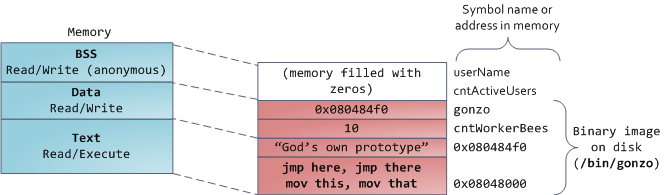
\includegraphics[width=.7\columnwidth]{mappingBinaryImage}
	\captionsource{Plan d'une image binaire dans les segments BSS, Data et Text}
	{Plan d'une image binaire dans les segments BSS, data et text, par G.~Duarte}
	{\url{http://duartes.org/gustavo/blog/post/anatomy-of-a-program-in-memory/}}
	\label{fig:mappingBinaryImage}
\end{figure}

\subsection{Descripteurs mémoires}

Lors de l'exécution d'un programme, cet espace mémoire est géré par le système d'exploitation grâce à des descripteurs de mémoire appelés \og memory descriptor \fg. Cette structure contient les adresses de début et de fin de chaque segments.

\begin{figure}[H]
	\centering
	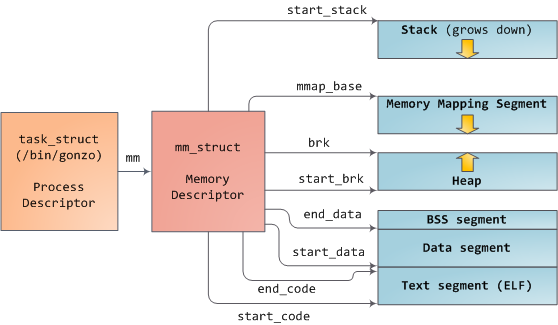
\includegraphics[width=0.5\columnwidth]{mm_struct}
	\captionsource{Descripteur de mémoire d'un processus Linux}
	{Descripteur de mémoire d'un processus Linux, par G.~Duarte}
	{\url{http://duartes.org/gustavo/blog/post/how-the-kernel-manages-your-memory/}}
	\label{fig:mm_struct}
\end{figure}

Cette structure globale est constituée d'une suite de plus petites structures appelées espaces virtuels de mémoire \og virtual memory area \fg, \mintinline{c}{vm_area_struct} sur la \autoref{fig:memoryDescriptorAndMemoryAreas}. Chacune d'elles est un espace continu en mémoire et permettent de stocker des informations tels que les droits d'écriture, de lecture ou encore les droits d'exécution du contenu mémoire. Elles stockent également si et quel fichier est mappé en mémoire.

\begin{figure}[H]
	\centering
	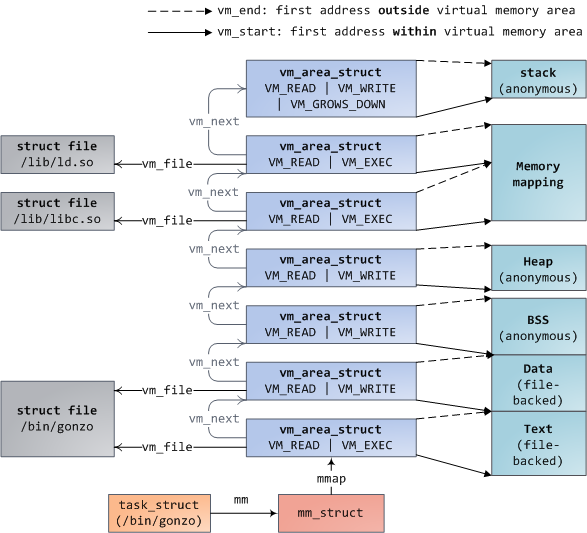
\includegraphics[width=0.7\columnwidth]{memoryDescriptorAndMemoryAreas}
	\captionsource{Structure des espaces virtuels de mémoire}
	{Structure des espaces virtuels de mémoire, par G.~Duarte}
	{\url{http://duartes.org/gustavo/blog/post/how-the-kernel-manages-your-memory/}}
	\label{fig:memoryDescriptorAndMemoryAreas}
\end{figure}

% ---------------------------------------------------------------------------
\section{\og Buffer overflow \fg}

Le dépassement de tampon, \og buffer overflow \fg en anglais, consiste à exploiter une fonction qui ne vérifie par la taille du contenu à copier en mémoire. En utilisant, par exemple, \mintinline{c}{strcpy()}, il est possible d'écrir sur l'adresse de retour de la fonction et ainsi modifier le flot de contrôle de l'application en le redirigeant à un endroit où l'attaquant aura, par exemple, préalablement injecté du code \og shellcode \fg.

\subsection{\og Stack frame \fg}

Une \og stack frame \fg permet de stocker toutes les informations nécessaires à l'exécution d'une fonction. Elle est créée sur la pile lors de l'appel de ladite fonction, par le prologue, et est détruite, avant l'appel de retour, par l'épilogue. Elle n'est pas détruite à proprement parlé, le pointeur \mintinline{c}{%ebp} est restauré dans son état précédent.

Lorsqu'une \og stack frame \fg est créée, celle-ci stocke dans un schéma particulier les informations dont elle a besoin. Les premières informations ont des adresses plus grandes en mémoires que les dernières, car la pile grandit de manière décroissante. La séquence suivante est exécutée à chaque prologue de fonction afin d'initialiser la \og frame \fg; sont placés sur la pile successivement:

\begin{enumerate}
	\item les paramètres passés à la fonction
	\item l'adresse de retour, équivalant à l'adresse de la fonction appelante
	\item une sauvegarde du pointeur \mintinline{c}{%ebp}, pour restaurer la \og frame \fg précédente lors de l'épilogue
	\item puis les variables locales, déclarées au sein de la fonction
\end{enumerate}

Le code d'exemple \autoref{lst:stack_example} contient une fonction \mintinline{c}{func()} qui est appelée avec deux arguments, \mintinline{c}{512} et \mintinline{c}{65536}, et qui déclare des variables locales. La \autoref{fig:stackIntro} illustre l'état de la pile à la fin de la ligne 6, avant le retour de la fonction.

\begin{listing}
	\cfile{02-main/listings/stack.c}
	\caption{Exemple de programme illustrant la gestion de la pile d'exécution}
	\label{lst:stack_example}
\end{listing}

Les deux arguments de 4~octets (en orange) sont d'abord mis sur la pile, l'adresse de retour ainsi que l'ancienne valeur de \mintinline{c}{%ebp} de 4~octets [adressage en 32~bits] (en bleu clair) sont ensuite sauvées, puis les deux variables locales, 4~octets pour l'entier et 8~octets pour le \mintinline{c}{local_buffer} (en vert à droite) sont crées.

\begin{figure}[H]
	\centering
	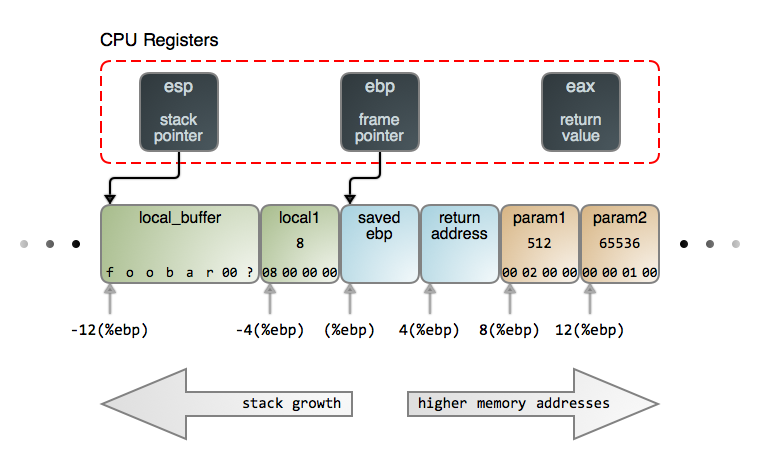
\includegraphics[width=0.6\columnwidth]{stackIntro}
	\captionsource{Exemple d'une Stack frame}
	{Exemple d'une structure de pile (Stack frame), par G.~Duarte}
	{\url{http://duartes.org/gustavo/blog/post/journey-to-the-stack/}}
	\label{fig:stackIntro}
\end{figure}

On constate alors que l'adresse de départ du \mintinline{c}{local_buffer} est inférieure de 16~octets à l'adresse stockant l'adresse de retour. Cette différence est déterministe et ne changera jamais lors de l'exécution.

\subsection{Exemple}

Grâce à cette structure, du fait que la pile grandit avec des adresses décroissantes ainsi que l'utilisation de fonction tel que \mintinline{c}{strcpy()}, il est possible, en dépassant la taille des variables locales, de modifier des zones mémoires telles que l'adresse de retour. Le code montré en \autoref{lst:buffer_example} permet d'illustrer un cas d'exploitation de la fonction \mintinline{c}{gets()} --- fonction vulnérable car elle ne s'arrête que lorsqu'elle rencontre un retour à la ligne ou un  \og \gls{eof} \fg \ ---.

\begin{listing}
	\cfile{02-main/listings/buffer.c}
	\caption{Exemple de programme illustrant un dépassement de tampon}
	\label{lst:buffer_example}
\end{listing}

En regardant la \autoref{fig:bufferCopy} on constate que si l'on écrit 28+4+4 octets = 36 octets dans le \mintinline{c}{buffer}, les 4 derniers octets auront écrasé l'adresse de retour.

\begin{figure}[H]
	\centering
	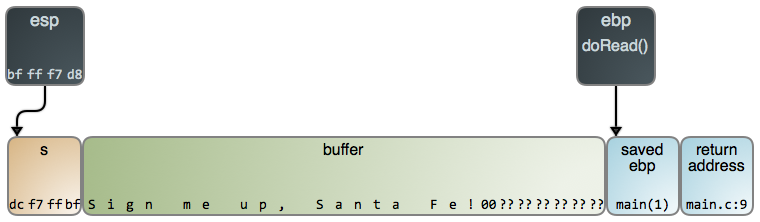
\includegraphics[width=0.8\columnwidth]{bufferCopy}
	\captionsource{Exemple de \og stack frame \fg avant un dépassement de tampon}
	{Exemple de \og stack frame \fg avant un dépassement de tampon, par G.~Duarte}
	{\url{http://duartes.org/gustavo/blog/post/epilogues-canaries-buffer-overflows/}}
	\label{fig:bufferCopy}
\end{figure}

Dans cette exemple, il est possible d'injecter un \og shellcode \fg dans le \mintinline{c}{buffer} grâce à la fonction \mintinline{c}{gets()}.

\begin{figure}[H]
	\centering
	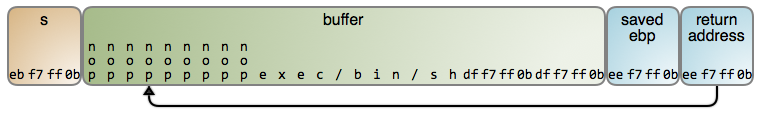
\includegraphics[width=0.8\columnwidth]{bufferOverflowExploit}
	\captionsource{Illustration de l'état de la pile au moment d'un dépassement de tampon}
	{Illustration de l'état de la pile au moment d'un dépassement de tampon, par G.~Duarte}
	{\url{http://duartes.org/gustavo/blog/post/epilogues-canaries-buffer-overflows/}}
	\label{fig:bufferOverflowExploit}
\end{figure}

\vfill

% ---------------------------------------------------------------------------
\section{DEP/NX}

Le mécanisme \gls{dep}/\gls{nx} a été mis en place pour éviter, lors d'un dépassement de tampon, que l'attaquant puisse exécuter du code stocké sur la pile. Les endroits mémoire censés contenir des données sont, via les \mintinline{c}{vm_area_struct} sous Linux, marquées comme étant non-exécutable. Le marquage indique ensuite au processeur, via le drapeau \gls{nx}, qu'il ne doit pas exécuter le contenu de cette plage mémoire.

\subsection{Mécanisme de protection}

Le mécanisme de Data Execution Prevention (\gls{dep}) a été introduit sur Linux en 2004 avec la version 2.6.8 du noyau, durant la même année pour Windows et deux ans plus tard pour Mac OS X, lors de la transition des puces PowerPC d'IBM vers l'architecture x86 d'Intel de 2006 à 2007 \cite{DataExecutionPrevention, PowerPC}.

La protection en soit se base sur le \og hardware \fg, le NX bit, introduit tout d'abord par AMD en 2003, puis repris par Intel sous le nom de \og XD bit \fg une année après \cite{ExecutableSpaceProtection, NXBit}. Ce bit indique au processeur s'il s'agit d'une zone d'instructions ou de données. Cette fonctionalité \og hardware \fg peut aussi être simulée, mais cela entraîne de ce fait une baisse de performance importante.

\subsection{Contournements grâce aux attaques \og return-to-libc \fg}

Une pile non-exécutable ne permet plus à l'attaquant d'exécuter son code, mais cela ne l'empêche pas d'exécuter du code marqué comme exécutable déjà présent au sein du programme ou des bibliothèques dynamiquements chargées. Comme montré dans l'exemple de la \autoref{fig:memoryDescriptorAndMemoryAreas}, la bibliothèque partagée \texttt{libc} est chargée en mémoire, ce qui est toujours le cas et ce qui rend une attaque de type \og return-to-libc \fg \cite{ReturntolibcAttack} possible.

Grâce à la fonction \mintinline{c}{system()} présente au sein de \texttt{libc}, il est possible d'exécuter arbitrairement un programme. Lors de l'attaque on localise, par exemple, une chaîne de caractères tel que \mintinline{c}{"/bin/sh"}, que l'on prépare comme étant le paramètre à passer à la fonction \mintinline{c}{system()}.

% ---------------------------------------------------------------------------
\section{ASLR}
\label{section:aslr}

Comme montré sur la \autoref{fig:mappingBinaryImage}, l'espace d'adressage virtuel est structuré de manière fixe. Les emplacements mémoires sont donc inchangés à chaque exécution du programme. De cette manière il est possible de prévoir où se trouve en mémoire les différents composants dont a besoin l'attaque. Une attaque de type \og return-to-libc \fg a besoin de connaître l'adresse de la fonction \mintinline{c}{system()} et de la chaîne de caractères \mintinline{c}{"/bin/sh"}. Dans le cas où ces adresses changent à chaque lancement, la tâche devient plus compliquée.

\subsection{Mécanisme de protection}

Depuis juin 2005, le mécanisme d'\og address space layout randomization \fg est supporté dans le noyau Linux avec la version 2.6.12 \cite{AddressSpaceLayoutRandomizationFR, AddressSpaceLayoutRandomizationEN}. Afin de rendre imprédictible les adresses sensibles, trois décalages aléatoires sont effectués au sein de la mémoire virtuelle. Le premier permet de décaler la pile vers le bas, le second décale lui aussi vers le bas le \og memory mapping segment \fg et le dernier décale vers le haut le segment du tas.

\begin{figure}[H]
	\centering
	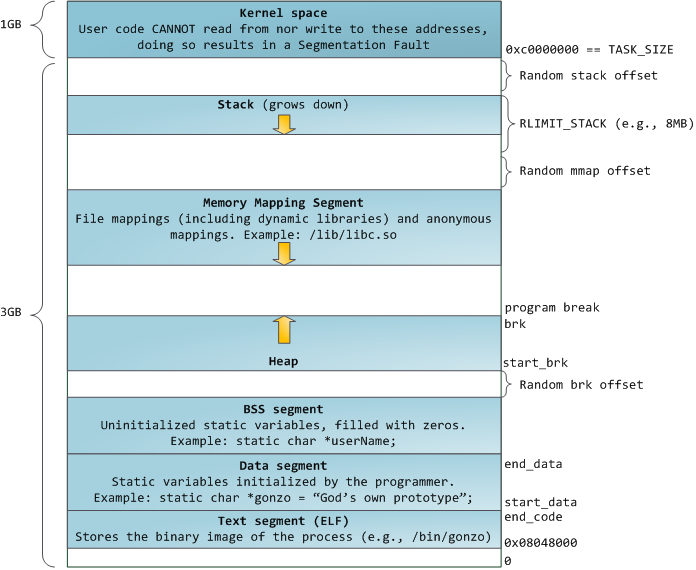
\includegraphics[width=1\columnwidth]{linuxFlexibleAddressSpaceLayout}
	\captionsource{Concept de l'address space layout randomization sous Linux en 32 bits}
	{Concept de l'address space layout randomization sous Linux en 32 bits, par G.~Duarte}
	{\url{http://duartes.org/gustavo/blog/post/anatomy-of-a-program-in-memory/}}
	\label{fig:linuxFlexibleAddressSpaceLayout}
\end{figure}

La \autoref{fig:linuxFlexibleAddressSpaceLayout} montre bien qu'en 32~bits, l'espace disponible n'est au total que de 4~Go, la part d'aléatoire est donc restreinte. À contrario, dans le cas d'un OS 64~bits \gls{aslr} devient bien plus intéressant, car l'espace mémoire virtuel est beaucoup plus vaste (256~To) sans que l'utilisation de celle-ci ne grandisse proportionnellement (au maximum 256~Go de mémoire sont affectés dans des cas classiques d'utilisation serveur). Il donc possible de décaler les segments de manière significative.

Malgré cela, les chercheurs Hector Marco-Gisbert et Ismael Ripoll de l'université de Valence ont écrit un papier démontrant une faiblesse d'\gls{aslr} en 64~bits sous certaines hypothèses \cite{EffectivenessFullASLR64bit}.

\subsection{Limitation et contournements}

Sur un OS 32 bits, la marge de manoeuvre laissée au décalage n'est pas très grande. Seule une partie des bits de l'adresse mémoire est utilisée, ce qui laisse possible à une attaque par recherche exaustive, exigeant quelques milliers d'essais seulement, d'aboutir. En effet la pile est placée aléatoirement avec une entropie de 19 bits seulement et le segment de \og memory mapping \fg avec 8~bits.

L'exemple \autoref{lst:bruteforce_aslr} montre comment avec un code Python d'une trentaine de lignes il est possible de faire une recherche exhaustive en 32 bits et d'exécuter un \og shellcode \fg dans un programme n'utilisant pas \gls{dep}/\gls{nx} et les \og \gls{stackCookies} \fg.

\begin{listing}
	\pythonfile{02-main/listings/aslrBruteforce.py}
	\caption{Exemple de recherche exhaustive en Python sur ASRL en 32 bits}
	\label{lst:bruteforce_aslr}
\end{listing}

Ce code est tiré du blog \og Sirius CTF \fg \cite{ExploitingSimpleBufferOverflow} et illustre l'utilisation de l'opération \mintinline{python}{"\x90"} indiquant au processeur de passer à l'instruction suivante. En définissant une taille de 4096 octets de \og \gls{nop} \fg on augmente drastiquement les chances de tomber sur le \og shellcode \fg. La \autoref{fig:bufferOverflowExploit} montre également l'état de la pile lors d'un dépassement de tampon avec utilisation de l'instruction \gls{nop}.

Le but premier d'\gls{aslr} est de venir contrer la prédictivité de l'emplacement des segments. On constate cependant que sur la \autoref{fig:linuxFlexibleAddressSpaceLayout}, aucun décalage n'est appliqué au segments \og BSS \fg, \og data \fg et \og text \fg, ce qui est tout à fait normal, \gls{aslr} ne modifie pas le segment \og text \fg. Malheureusement cela laisse la prédictibilité de l'emplacement du code exécutable et ouvre la porte à de nouvelles attaques, par exemple de type \og \gls{rop} \fg. Il existe d'autres mécanismes, tel que \og \gls{pie} \fg \cite{PositionIndependentExecutables}, vennant appliquer de l'aléatoire sur certaines partie du code et des bibliothèques. Mais ces mécanismes ne sont pas décrit dans ce rapport.

\vfill

% ---------------------------------------------------------------------------
\section{\og Stack canaries \fg}

Les \og \gls{stackCanaries} \fg ou \og \gls{stackCookies} \fg sont des valeurs déposées sur la pile d'exécution, après la valeur de retour, lors de l'appel d'une fonction. Le nom \og canaries \fg vient par analogie aux canaris que l'on plaçait dans le mine pour prévenir les fuites de monoxyde de carbone \cite{StackCanaries, SentinelSpecies}. Ces oiseaux étant petits et vite atteints par les effets du gaz, ils donnaient rapidement l'informations aux mineurs qu'un danger était présent.

Le fonctionnement des \og \gls{stackCanaries} \fg est pareil, la valeur du canari est vérifiée lors de l'épilogue de la function et, si celle-ci ne correspond pas à la valeur du canari d'origine, alors une tentative de dérouter le flot de contrôle de l'application est détectée et l'on peut alors réagir en conséquence \cite{EpiloguesCanariesBufferOverflows}.

\begin{figure}[H]
	\centering
	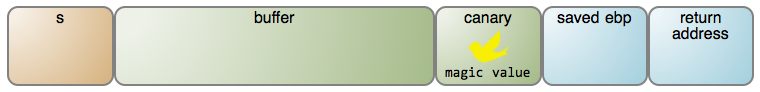
\includegraphics[width=1\columnwidth]{bufferCanary}
	\captionsource{Illustration de l'état de la pile protégée par un canari}
	{Illustration de l'état de la pile protégée par un canari, par G.~Duarte}
	{\url{http://duartes.org/gustavo/blog/post/epilogues-canaries-buffer-overflows/}}
	\label{fig:bufferCanary}
\end{figure}

\subsection{Implémentation}

Il existe trois types principaux de canaris: \og \textit{terminator} \fg, \og \textit{random} \fg, et \og \textit{random XOR} \fg \cite{BufferOverflowProtection}. Les \og \textit{terminator canaries} \fg se base sur le constat que l'exploitation d'un dépassement de tampon est une opération sur une chaîne de caractères. De ce fait, si le canari est constitué de caractères tels que \mintinline{c}{null}, \mintinline{c}{CR}, \mintinline{c}{LF} ou encore \mintinline{c}{-1}, alors la fonction \mintinline{c}{strcpy()} ou \mintinline{c}{gets()} se terminera avant de réécrire l'adresse de retour. Le désavantage notable de cette méthode se retrouve dans le fait que l'attaquant connaît la valeur du canari.

Le \og \textit{random canary} \fg est tiré aléatoirement afin de palier au problème du \og \textit{terminator canary} \fg. Généralement ce canari est généré à l'initialisation du programme et est stocké dans une variable globale.

Le \og \textit{random XOR canary} \fg est une méthode un peu plus élaborée, elle fonctionne de la même manière que le \og \textit{random canary} \fg mais est en plus calculée en fonction de tout ou partie du programme, ce qui rend encore plus difficile pour l'attaquant de forger un canari valide.

L'application de la protection par canaries au sein de \gls{clang}/\gls{llvm} peut se faire grâce au composant \og StackProtector \fg \cite{LLVMStackProtector}. Ce composant effectue une analyse lors de la compilation, couplée à l'utilisation d'une librairie lors de l'exécution.

\subsection{Limitation et contournements}

Dans les deux premières implémentations --- \og \textit{terminator canaries} \fg et \og \textit{random canaries} \fg \ ---, il est possible de contourner les canaris en récupérant leur valeur. Ce qui peut être fait directement sur la pile d'exécution grâce au contrôle, par exemple, des paramètres d'une fonction tel que \mintinline{c}{printf()} qui nous permet de lire en mémoire grâce au format \mintinline{c}{%p}.

Dans le cas d'un \og \textit{random XOR canary} \fg, si l'adresse de retour est modifiée, alors la valeur du canari change, car elle dépend de la valeur aléatoire de départ et des données sur la pile d'exécution. L'exploitation devient alors plus complexe à mettre en place mais reste possible.

% ---------------------------------------------------------------------------
\section{\og Control-flow integrity \fg}

\gls{cfi} est un concept permettant, par analyse statique, de définir les changements possibles du flot de contrôle de l'application, appelé \og \gls{cfg} \fg, pour ensuite valider ou non le changement effectif lors de l'exécution du programme. Le papier original démontrant l'approche \cite{CFIPaper}, publié en 2005, est généralement attribué au centre de recherche de Microsoft. Depuis, de nombreux papiers ont été publiés améliorant les performances ou modifiant légèrement l'approche.

Actuellement le concept de \gls{cfi} est implémenté au sein de \gls{clang} sous le nom de \og forward-edge CFI \fg \cite{ControlFlowIntegrity, TalkAboutCFIClang, ControlFlowIntegrityDesignDocumentation}. Dans la documentation dédiée, un example de coût en performance de 15\% est relevé sur Chromium. On peut également constater, dans d'autre sources de la litérature, que l'approche classique impose un coût de 16\% en moyenne et de 45\% dans le pire des cas \cite{ControlFlowIntegrityMaryland}. Ce qui en fait la principale faiblesse de cette approche.

Les principales variations du concept se font sur la granularité choisie lors de la construction du \gls{cfg}. Deux \og modèles \fg émèrgent et se généralisent: \og \gls{fg-cfi} \fg et \og \gls{cg-cfi} \fg.

\subsection{\og Fine-grained CFI \fg}

La variation \og \gls{fg-cfi} \fg \cite{FineCFI, FineCFIKernel}, comme son nom l'indique, a une approche précise lors de la construction du \gls{cfg}. Chaque élément du graphe est labélisé de manière précise et lors de l'exécution du programme, à chaque changement du flot de contrôle on vérifie si la destination labélisée correspond à un label voisin de l'élément de départ. Cependant cette manière de faire amène, par ces nombreuses vérifications, un coût important en terme de performances.

\subsection{\og Coarse-grained CFI \fg}

La variation \og \gls{cg-cfi} \fg est une approche plus simple quant à la labélisation du \gls{cfg},  et donc plus performante, mais ouvrant la porte à certaines faiblesses. Les points de contrôle de l'application son labélisés de manière à obtenir un nombre restreint de labels. Ceux-ci sont alors réutilisés au sein du même graphe, de ce fait il est possible de partir d'un point A et aller au point C alors que cela n'est pas prévu, mais par cause d'une labélisation non unique l'erreur n'est pas détectée.

\newpage

\section{Résumé}

Il existe à ce jour une multitude de concepts ayant pour mission d'entraver ou de ralentir les attaques visant le flot de contrôle d'une application. Ces concepts ne gèrent, individuellement, qu'une partie de la problématique et sont donc généralement appliqués conjointement. Aujourd'hui, il n'existe pas encore de mécanismes permettant de garantir seul, à 100\%, l'intégrité du flot sans engager des coûts trop importants en performance, rendant leur utilisation impossible dans un environnement de production. Tous les mécanismes de protection passés en revue peuvent être contourné par une attaque évoluée de type \gls{rop}.

Le papier présentant CPI/CPS/SafeStack \cite{CPIPaper} et son prototype appelé \gls{levee} promettent un mécanisme permettant de contrer ce type d'attaque et à moindre coût. Afin d'y parvenir, l'équipe de chercheurs à mis en place différents concepts se raprochant de ce qui se fait au sein des languages de programmation de type \og memory-safe \fg. En effet, les implémentations actuelles permettant de garantire à 100\% le flot de contrôle --- SoftBound+CETS --- sont une application directe des concepts présent au sein des languages de type \og memory-safe \fg aux languages \texttt{C/C++}. Cependant cette application directe n'est pas viable en terme de performances. Les chercheurs du projet \gls{levee} ont alors proposé d'appliquer ces méthodes sur une partie spécifique du programme.

% \newpage

% % -------------------------------------------------------------------------
% This chapter shows example of picture and also serves to populate the different lists: list of figures, list of tables, bibliography, and glossary.
%
% \section{Tables}
%
% This section contains an examples of table: \autoref{tab:esempio}
%
% \begin{table}[H]
% 	\centering
% 	\begin{tabular}{ccc}
% 		\toprule
% 		name & weight & food \\
% 		\midrule
% 		mouse	& 10 g	& cheese \\
% 		cat	& 1 kg	& mice \\
% 		dog	& 10 kg	& cats \\
% 		t-rex	& 10 Mg	& dogs \\
% 		\bottomrule
% 	\end{tabular}
% 	\caption[A floating table]{A floating table.}
% 	\label{tab:esempio}
% \end{table}
%
% \section{Figures}
%
% This section contains examples of figures: \autoref{fig:galleria}, \autoref{fig:lorem}, \autoref{fig:ipsum}, \autoref{fig:dolor}, \autoref{fig:sit}
%
% \begin{figure}[H]
% 	\centering
% 	\includegraphics[width=0.5\columnwidth]{galleria_stampe}
% 	\captionsource{A floating figure}{A floating figure: the lithograph \emph{Galleria di stampe}, of M.~Escher}{\url{http://www.mcescher.com/}}
% 	\label{fig:galleria}
% \end{figure}
%
% \begin{figure}[H]
% 	\centering
% 	\begin{subfigure}[b]{0.45\textwidth}
% 		\includegraphics[width=\textwidth]{lorem}
% 		\caption{A gull}
% 		\label{fig:lorem}
% 	\end{subfigure}
% 	~ %add desired spacing between images, e. g. ~, \quad, \qquad, \hfill etc.
% 	%(or a blank line to force the subfigure onto a new line)
% 	\begin{subfigure}[b]{0.45\textwidth}
% 		\includegraphics[width=\textwidth]{ipsum}
% 		\caption{A tiger}
% 		\label{fig:ipsum}
% 	\end{subfigure}
% 	~ %add desired spacing between images, e. g. ~, \quad, \qquad, \hfill etc.
% 	%(or a blank line to force the subfigure onto a new line)
% 	\begin{subfigure}[b]{0.45\textwidth}
% 		\includegraphics[width=\textwidth]{dolor}
% 		\caption{A mouse}
% 		\label{fig:dolor}
% 	\end{subfigure}
% 	~ %add desired spacing between images, e. g. ~, \quad, \qquad, \hfill etc.
% 	%(or a blank line to force the subfigure onto a new line)
% 	\begin{subfigure}[b]{0.45\textwidth}
% 		\includegraphics[width=\textwidth]{sit}
% 		\caption{A mouse}
% 		\label{fig:sit}
% 	\end{subfigure}
% 	\caption{Example subcaption}\label{fig:animals}
% \end{figure}
%
%
% % -----------------------------------------------------------------------------
% \section{Code}
%
% \autoref{lst:listing_example} shows an example of Java code rendered with minted.
%
% \begin{listing}
% 	\javafile{02-main/listings/HelloWorld.java}
% 	\caption{Example of listing using the minted package}
% 	\label{lst:listing_example}
% \end{listing}
%
% % -----------------------------------------------------------------------------
% \section{Other features}
%
% Term (glossaries): \gls{nosql}
%
% Acronym (glossaries): \gls{sql}
%
% Citation (biblatex): \cite{paper_millwheel}
%
% % -----------------------------------------------------------------------------
% \section{Conclusion}
%
% \blindtext

\chapter{Analyse de Levee}
\label{chap:levee}

% introduction du projet Levee... composant, équipe, epfl

\gls{levee} est un projet mené dans le cadre du Dependable Systems Lab \cite{dslab} par les chercheurs Volodymyr Kuznetsov, Laszlo Szekeres, Mathias Payer, George Candea, R. Sekar et Dawn Song. Le but annoncé du projet est de sécuriser tout programme informatique contre la totalité des attaques de type \og control-flow hijack \fg via une erreur mémoire, du moment où celui-ci a été compilé grâce à \gls{clang} avec les options nécessaires.

Comme montré dans le chapitre précédent, il existe déjà plusieurs mécanismes (\gls{dep}, \gls{aslr}) permettant de réduire le risque de ce type d'attaque sans imposer au programme de coût supplémentaire en matière de performance. Cependant, il est aujourd'hui possible de les contourner, même au sein d'un environnement de production, grâce à des attaques évoluées telles que le \gls{rop}. D'autres mécanismes plus évolués (\gls{cfi}, SoftBound+CETS, CCured ou encore AddressSanitizer) permettent quant à eux d'améliorer trés fortement la sécurité, mais ne permettent pas, soit de garantir une totale intégrité et reste à ce jour contournable, soit ils ne sont pas adoptés à grande échelle à cause de leurs effets beaucoup trop négatifs sur la performance du programme --- jusqu'à 116\% de coût en performance ---.

Le défi relevé par l'équipe de recherche a été de proposer un modèle de sécurité entrainant des coûts faibles en matière de performance tout en garantissant l'intégrité complète du flot de contrôle. \gls{levee} est le prototype d'implémentation de ce modèle et ce chapitre se concentre sur ses aspects théoriques, son implémentation au sein des outils de compilation \gls{llvm} et son rayon d'action.

\minitoc

\newpage

% -----------------------------------------------------------------------------
\section{Concepts théoriques}

Seules les attaques visant à dérouter le flot de contrôle de l'application sont prises en compte dans le modèle de sécurité. Les attaques du types \og data-only \fg, visant à modifier ou récupérer des informations qui ne font pas partie du flot, n'entrent pas en considération.

Ils émettent l'hypothèse que l'attaquant a le contrôle total sur la mémoire du processus et que le chargement du programme ainsi que le binaire ne peuvent pas être altérés. De ce fait, les mécanismes de protection résultant de la compilation peuvent se mettre en place avant l'intervention de l'attaquant.

Les chercheurs du projet posent comme postulat de départ qu'il est suffisant de garantir l'intégrité des pointeurs pour rendre impossible la modification du flot de contrôle via exploitation d'erreurs mémoires. Dans le cas des langages de types \og memory-safe \fg, un objet en mémoire ne peut être accédé que depuis un pointeur prévu explicitement pour l'objet en question. Cela rend la modification du flot de contrôle impossible, mais entraîne une baisse de performances importante.

Afin de garder de bonnes performances tout en garantissant l'intégrité complète, le minimum d'instrumentation doit être délégué à l'exécution. Le code est alors en premier lieu analysé de manière statique à la compilation, puis des mécanismes de vérification sont ensuite délégués à l'exécution. Le concept de \og \gls{cpi} \fg \cite{CPIPaper} intervient alors, afin de déterminer quels pointeurs doivent être protégés, ce qui permet de réduire au minimum les accès à controler lors de l'exécution.

\section{CPI (Code-pointer integrity)}

% Decrire pourquoi les pointeurs sensibles et pas sensibles. comment determiner si un pointeur est sensible

\subsection{Définition d'un \og code-pointer \fg}

Afin de formaliser les pointeurs de code (code-pointers), le papier propose la définition suivante :

On dit que l'indirection ou le déréférencement d'un pointeur est sûr si et seulement si l'adresse mémoire à laquelle il tente d'accéder est comprise au sein de l'\textit{objet mémoire} sur lequel le pointeur est \textit{basé}. Un \textit{objet mémoire} est une abstraction liée au langage définissant tout types de structures stockées en mémoire (variables globales, variables locales, structures, objets), de sous-structures (un champ d'une structure) ou encore des points de contrôle du flot (adresse de départ d'une fonction, adresse de retour). Ces \textit{objets mémoires} ont un cycle de vie défini, lorsqu'on libére la mémoire liée à un tableau et qu'on alloue un nouveau tableau avec la même adresse, un nouvel \textit{objet mémoire} est créé.

Le papier formalise ensuite la définition de pointeur \textit{basé sur} un \textit{objet mémoire}. On dit qu'un pointeur est \textit{basé sur} sur un \textit{objet mémoire X} si et seulement si le pointeur est obtenu lors de l'exécution par (i) allocation de \textit{X} sur la pile, (ii) référencement explicit de l'adresse de \textit{X}, (iii) en référencant l'adresse d'un sous-objet \textit{y} de \textit{X} (accès au champ \textit{y} d'une structure \textit{X}), ou (iv) en effectuant une expression sur un pointeur (calculs arithmétiques, position au sein d'un tableau, copie de pointeur) impliquant l'adresse de l'\textit{objet mémoire X}. Cette définition est basée sur la définition des pointeurs \textit{basé sur} présente au sein de la norme \texttt{C99}.

\newpage

Si l'on part maintenant du principe que ces deux définitions sont strictement respectées pour tout pointeurs, peu importe les paramètres donnés à l'exécution du programme, alors on peut qualifier le-dit programme de \textit{memory-safe}. Dans ce cas il n'est plus possible de dérouter le flot de contrôle en exploitant une erreur basée sur la mémoire.

\subsection{Concept théorique}

Le mécanisme de \gls{cpi} est statisfait si toutes les indirections ou les déréférencements sur les pointeurs accédant ou déréférençant des pointeurs jugés \og sensibles \fg sont sûrs. La définition des pointeurs jugés sensibles est donc récursive. Les pointeurs de départ devant être protégés sont les pointeurs responsables de transférer le flot de contrôle de l'application. Cette notion de récursivité est donc dynamique, un pointeur de type \mintinline{c}{void*} doit être considéré comme sensible s'il pointe vers une fonction ou sur un autre pointeur jugé sensible, mais ne doit pas être considéré comme sensible s'il pointe vers un type \mintinline{c}{int}.

Les langages de programmation bénéficiant d'une mémoire supervisée satisfont le concept de \gls{cpi}. Cependant, ils ne différencient pas les pointeurs sensibles des autres, ce qui entraîne une forte baisse de performance par rapport aux langages de type \texttt{C/C++} (le papier mentionne une perte de $\geq2\times$ au sein des meilleures implémentations actuelles).

L'observation faite par l'équipe de chercheurs est la suivante: afin de garantir le flot de contrôle de l'application, seul l'accès aux pointeurs jugés sensibles doit être vérifié et ces pointeurs forment un ensemble de petite taille sur l'ensemble des pointeurs. Les pointeurs agissant sur les données peuvent se permettre de ne pas être controlés, ce qui augmente l'efficacité tout en maintenant un très haut taux de protection.

\subsection{Déterminer l'ensemble des pointeurs sensibles}

Afin de déterminer l'ensemble des pointeurs devant être considérés comme sensibles, une analyse statique est effectuée. Pour ce faire une heuristique simple est utilisée: \og un pointeur est jugé sensible si son type est sensible \fg. Les types marqués comme étant sensibles sont:

\begin{enumerate}
	\item pointeurs de fonction
	\item pointeurs vers des pointeurs sensibles
	\item pointeurs vers des types composés (\mintinline{c}{array}, \mintinline{c}{struct}) qui contiennent un ou plusieurs pointeurs sensibles
	\item pointeurs universels (\mintinline{c}{void*}, \mintinline{c}{char*})
  \item pointeurs explicitements créés par le compilateur ou à l'exécution (adresse de retour, tables virtuelles en C++ \cite{fonctionsVirtuelles}, \mintinline{c}{setjmp} \cite{setjmp})
\end{enumerate}

Cet ensemble de types peut être adapté, étendu, suivant les besoins du programme ou de la plateforme. Le papier mentionne en exemple la structure \mintinline{c}{ucred} utilisée dans le noyau FreeBSD, qui est marquée comme sensible car elle contient les UIDs des processus et d'autres informations.

En effectuant des tests, les chercheurs se sont rendu compte que l'analyse heuristique mettait en avant un ensemble de pointeurs correspondant en moyenne à $6.5\%$ de l'ensemble global. Ce chiffre met en avant l'impact sur l'efficacité qu'a cette approche.

Le coût en performance dépend directement de l'heuristique et de sa récursion. L'équipe mentionne elle-même que toutes heuristiques donnant un ensemble approximatif cohérent peuvent être utilisées. Des améliorations peuvent encore être attendues sur ce point. Le second avantage majeur de cette approche réside dans le fait que l'on peut facilement imaginer de nouvelles heuristiques permettant de protéger d'autres ensembles de pointeurs, par exemple, pour protéger une partie des données au sein du programme.

\subsection{Zone de mémoire sûre \og safe region \fg}

Afin de garantir l'intégrité de l'ensemble des pointeurs sensibles, une zone mémoire appelée \og \textit{safe region} \fg est créée, voir la \autoref{fig:safeRegionLayout}. Cette région est isolée et ne peut être accédée que via des instructions fournies par \gls{cpi}. Cela permet de garantir l'intégrité des données et la propagation des métadonnées. Elle est ensuite constituée d'un \og \textit{safe pointer store} \fg, pour les pointeurs sensibles, et de \og \textit{safe stacks} \fg, pour une gestion plus spécifique liée à la pile d'exécution, voir la \autoref{section:safeStack}. Seule l'une des deux copies présente dans les deux régions est utilisée suivant le type du pointeur en question.

\begin{figure}[H]
	\centering
	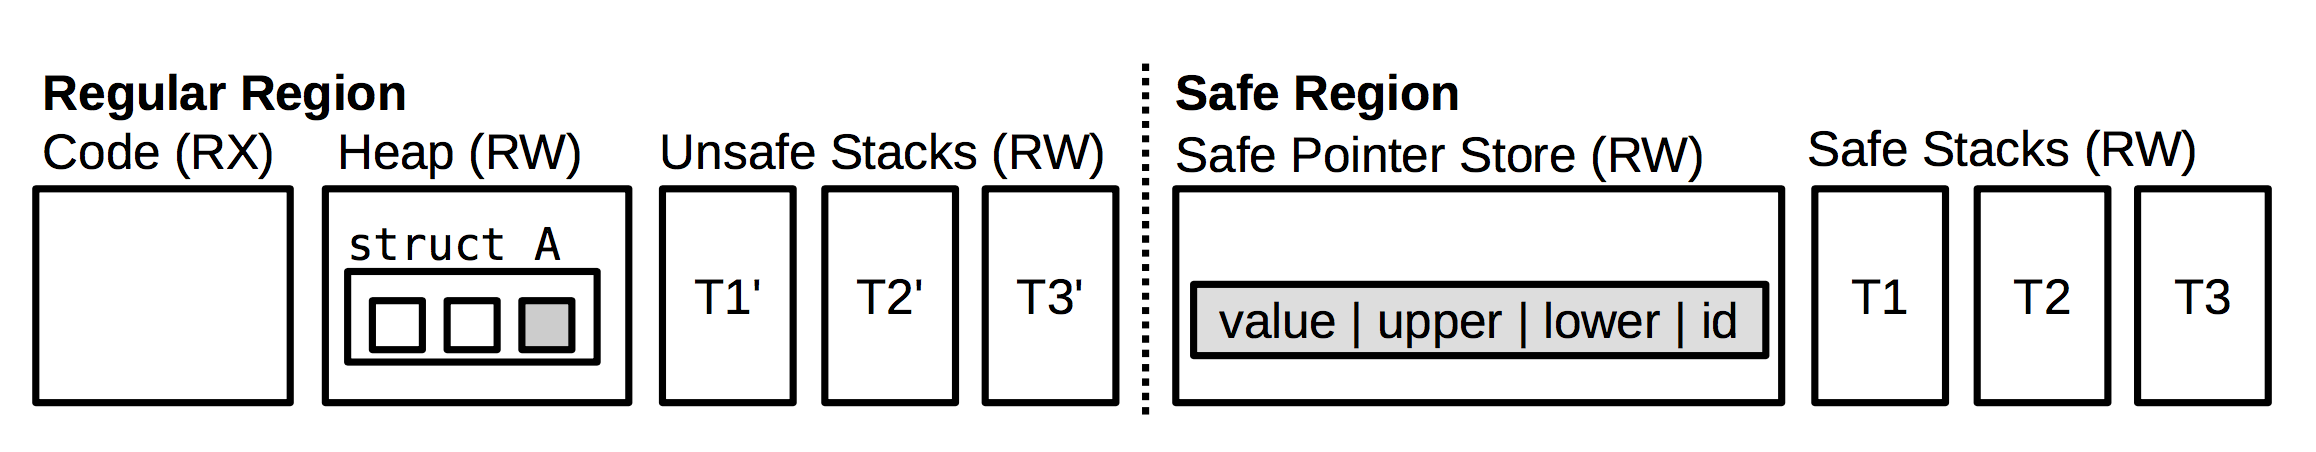
\includegraphics[width=1\columnwidth]{safeRegionLayout}
	\captionsource{Agencement de la mémoire avec CPI}
	{Agencement de la mémoire avec CPI, tiré du papier Code-Pointer Integrity}
	{\url{http://dslab.epfl.ch/pubs/cpi.pdf}}
	\label{fig:safeRegionLayout}
\end{figure}

Le \textit{safe pointer store} permet de stocker la valeur du pointeur et les métadonnées de l'\textit{objet mémoire} sur lequel le pointeur est \textit{basé}. Les métadonnées sont constituées de l'adresse de départ et de fin de l'objet au sein de la mémoire standard ainsi que d'un identifiant temporaire de l'objet en question. L'approche est similaire à celle utilisée au sein de SoftBounds+CETS \cite{SoftBound} à la différence prêt que \gls{cpi} stocke également la valeur du pointeur et n'applique pas de protection sur tout les pointeurs du programme.

\gls{cpi} garantit (i) que tous les pointeurs sensibles sont stockés dans la \og \textit{safe region} \fg, (ii) que la création et la modification lors de l'exécution de pointeurs sensibles soit propagée et (iii) que toutes les indirections ou les déréférences soient vérifiées grâce au métadonnées. Afin d'y parvenir, \gls{cpi}, lors de la phase de compilation, réécrit les instructions de création et d'accès de l'ensemble des pointeurs sensibles.

% on stocke l'adresse du pointeur dans la région standard ainsi que ca valeur = deux adresses
% TODO figure montrant qu'est ce qui est stocké et les liens

\subsection{Isolation de la zone de mémoire sûre}

Une fois les metadonnées et les \og \textit{safe stacks} \fg placées au sein de la région sûre, il faut pouvoir garantir leur intégrité. Pour ce faire cette région doit être isolée du reste de la mémoire et il ne doit pas être possible de la modifier sans passer par les instructions fournies par \gls{cpi}. Ce mécanisme de protection est directement dépendant de l'architecture pour laquelle le binaire est compilé. Dans les deux cas, la région sûre est placée dans le segment de \og memory mapping \fg avec un accès en lecture et écriture.

\subsubsection{Architecture 32~bits}

Dans le cas d'une architecture \texttt{x86-32}, la \og \textit{safe region} \fg est isolée grâce à l'utilisation des segments mémoires. Un segment mémoire n'étant pas utilisé au sein du programme est utilisé par \gls{cpi} afin de stocker l'adresse de base de la \og \textit{safe region} \fg. Les autres segments sont configurés afin de rendre l'accès à la région sûre impossible.

% \textit{TODO définition des segments, exemple d'utilisation etc... tout la sécu se base la dessus. Sinon ca revient à de l'ASLR}

La preuve de sécurité sous cette architecture repose sur le fait qu'il n'est pas possible, lors de l'exécution, d'atteindre ou de modifier le segment qui contient la région de mémoire sûre.

\subsubsection{Architecture 64~bits}

Au sein d'une architecture \texttt{x86-64} la limitation des segments n'est plus présente, mais l'architecture met toujours à disposition deux registres de segments mémoire. \gls{cpi} utilise l'un des deux segments pour stocker l'adresse mémoire de base pour la \og \textit{safe region} \fg. Cette adresse de base est tirée aléatoirement lors du lancement de l'application, ce qui ressemble fortement à l'approche d'\gls{aslr} expliquée en \autoref{section:aslr}. Cependant, la différence mentionée dans le papier est qu'il n'existe aucun pointeur vers la \og \textit{safe region} \fg au sein de la région standard, ce qui fait qu'il n'est pas possible de remonter jusqu'à l'adresse de base. Les 48~bits d'adressage offrent donc une sécurité suffisante et rendent impraticable une attaque par recherche exhaustive.

La preuve de sécurité, sous architecture \texttt{x86-64}, est donc basée sur des informations cachées. Ils mentionnent le fait que leur modèle est \og leak-proof \fg \ --- c’est-à-dire qu'il ne laisse pas fuiter d'informations concernant la localisation de la région sûre ---, à la différence d'\gls{aslr}, grâce à l'absence de pointeur vers la \og \textit{safe region} \fg lors de l'execution.


\section{CPS (Code-pointer separation)}

% Decrire la variante CPS, moins d'overhead mais permettant certain hijack

Les chercheurs se sont rendus compte que dans le cas du \texttt{C++}, l'ensemble des pointeurs sensibles peut rapidement devenir trop important pour cause, par exemple, d'utilisation de fonctions virtuelles. Tous les pointeurs vers un objet contenant une fonction viruelle deviennent alors sensibles, ce qui peut induire un coût de performance trop élevé. Pour palier à ce problème, le concept de \og \gls{cps} \fg a été mis en place. L'idée est de modifier quelque peu l'approche et de baisser les coûts en performance tout en garantissant le flot de contrôle.

Pour y arriver, l'heuristique utilisée pour définir l'ensemble des pointeurs lors de l'analyse statique ainsi que la définition d'un pointeur \textit{basé sur} sont modifiées. Seul les pointeurs pointant directement sur une destination du flot de contrôle sont protégés, laissant la récursion de côté. Contrairement à l'approche \gls{cpi}, il est possible de ne pas stocker de métadonnées dans la zone de mémoire sûre, en effet, en évitant par exemple les pointeurs sur des objets, chaque pointeur doit alors correspondre exactement à l'adresse de destination, les bornes ne sont plus nécessaires.

Les accès mémoires prennent alors, dans la majeur partie des cas (excepté pour les pointeurs de type universel), la même quantité de ressources qu'un programme sans \gls{cps}, à la différence que les pointeurs sensibles sont accédés et stockés dans la région sûre à la place de leur emplacement original.

\newpage

Les chiffres avancés au niveau des gains en performance de \gls{cps} sont de l'ordre de $4.3\times$ plus rapide que \gls{cpi}. Le coût mesuré passe alors de $8.4\%$ à $1.9\%$. Évidemment ces chiffres dépendent de l'ensemble des pointeurs à protéger et donc dirrectement de l'architecture dudit programme.

\section{Safe Stack}
\label{section:safeStack}

% quel est le concept de la safe stack

% -----------------------------------------------------------------------------
\section{Implémentation au sein de LLVM}

% version de LLVM, depuis quand, sous quel nom, documentation
%
% structure de LLVM front-end, l'optimizer, et le back-end, son fonctionnement, origine

\subsection{Structure de LLVM}


\subsection{Architecture de Levee}

% description des actions effectuée dans le front-end, l'optimizer, et le back-end

% -----------------------------------------------------------------------------
\section{Rayon d'action}

% qu'est qu'il est sensé proteger par rapport au chapitre historique

\chapter{Proof of concept d'une attaque}
\label{chap:attaque}

L'implémentation de \og \gls{safeStack} \fg au sein de \gls{llvm} doit permettre de prévenir les attaques se basant sur l'éxploitation d'un dépassement de tampon. Dans ce chapitre un \og proof of concept \fg d'une telle attaque est décrit sur un exemple de code fictif. Afin de rendre plus portable et reproductible cette phase de test, un environnement spécifique est mis en place et décrit précisément ainsi que la recette utilisée lors de la phase de compilation.

L'objectif est de démontrer l'efficacité de \gls{levee} et de comparer l'approche avec celle des \og \gls{stackCookies} \fg. Pour ce faire, une première attaque a été pensée, malheureusement celle-ci n'avais pas la possibilité d'aboutir. Basée sur ces conclusions, une autre attaque a été mise en place. Leur descriptions théorique ainsi que leurs implémentations sont décrites dans ce chapitre.

Un des exemples d'attaque proposé dans ce chapitre est basé sur l'article \og Introduction to return oriented programming (ROP) \fg du blog \textit{codearcana.com} \cite{IntroductionToROP}.

\minitoc

\newpage

% -----------------------------------------------------------------------------
\section{Environnement}

Afin de faciliter la mise en place de l'attaque, la compilation est faite en 32~bits. L'environnement choisi pour installer la version 4.0 de \gls{llvm} est Debian 8 en 64~bits. Afin de pouvoir correctement compiler et exécuter en 32~bits, les bibliothèques nécessaires doivent être installées (lignes 20 à 22). En plus de \gls{llvm}, \gls{gdb} ainsi que quelques autres utilitaires sont installés.

\subsection{Docker}

L'environnement décrit ci-dessus ainsi que l'installation des outils sont mis en place grâce à Docker. Le Dockerfile suivant contient toutes les instructions nécessaires afin d'installer la version 4.0 de \gls{llvm} et \gls{clang}.

\begin{listing}
	\dockerfile{02-main/listings/Dockerfile}
	\caption{Fichier décrivant l'environnement choisi pour l'installation de \gls{llvm} 4 sous Debian 8}
	\label{lst:dockerfile}
\end{listing}

Il existe plusieurs manières d'installer \gls{llvm}. Il serait tout à fait possible de compiler directement depuis les sources. Plusieurs de ces techniques ont été testées, et la suivante a été retenue: l'installation de Clang 4.0, \gls{lldb} (équivalant de \gls{gdb}) et de LLD (le \og linker \fg de \gls{llvm}) se fait en rajoutant le dépôt APT de \gls{llvm}. Après plusieurs essais, le débogueur \gls{gdb} est préféré à \gls{lldb} et est par la suite utilisé à la place de \gls{lldb}, ce dernier n'étant pas encore assez complet et globalement utilisé.

Tout les autres fichiers de configurations de l'environnement Docker sont disponibles à l'annexe \ref{chap:dockerConf}.

\subsection{Gestion de la compilation}

L'utilitaire \textit{make} est utilisé pour gérer le processus de compilation. Un Makefile est mis en place afin de rassembler les différents \og flags \fg utilisés pour générer les deux versions exécutables (l'un avec \gls{safeStack} et l'autre sans). En en-tête, différentes variables utilisées par \textit{make} sont définies afin de s'assurer que \gls{clang} 4.0 est bien utilisé. Deux version de l'exécutable sont créés: \textit{safe-stack} et \textit{stack-cookie}. Le language intermédiaire de \gls{llvm} est émis lors de la compilation afin de comparer les effets de l'un et l'autre mécanisme de protection.

À noter que la protection de la pile \texttt{\textit{-fstack-protector}} est desactivée grâce à \texttt{\textit{-fno-stack-protector}} lorsque l'on active \og \gls{safeStack} \fg. Le but étant de comparer les deux mécanismes, qui plus est, actuellement \og \gls{safeStack} \fg n'est pas compatible avec les \og \gls{stackCookies} \fg.

\begin{listing}
	\makefile{02-main/listings/Makefile}
	\caption{Makefile regroupant les différentes options de compilations}
	\label{lst:defaultMakefile}
\end{listing}

Un script permettant d'afficher les mécanismes de protection d'un binaire est utilisé, pour cela une règle spécifique aux tests est décrite à la ligne 38.

\vfill

\subsection{Mécanismes de sécurité actifs}

\gls{aslr} est actif au sein de l'environnement. Chaque binaire est protégé soit avec \og \gls{stackCookies} \fg ou avec \og \gls{safeStack} \fg. Le script \mintinline{bash}{checksec.sh} \cite{CheckSec} est utilisé pour afficher les mécanismes actifs sur chaque binaire. On peut constater sur le résultat ci-dessous que les \og \gls{stackCookies} \fg sont bien désactivés lors du test de \og \gls{safeStack} \fg et que dans les deux cas le drapeau \gls{nx} est actif.

\begin{listing}
	\textfile{02-main/listings/checksec.res}
	\caption{Resultat du test de sécurité par checksec.sh}
	\label{lst:checksecRes}
\end{listing}

\gls{pie} est un mécanisme de protection récent qui permet d'appliquer de l'aléatoire sur des régions de code, et ainsi rendre plus difficile la mise en place d'une attque de type \gls{rop}.


% -----------------------------------------------------------------------------
\section{Pointeur de fonction sur la pile}

\subsection{Description théorique de l'attaque}

La première tentative se base sur une \textit{structure} dans laquelle est stocké un pointeur vers une fonction. En plaçant la \textit{structure} et le tampon sur la pile d'exécution, l'idée est de réécrire l'adresse du pointeur présent dans ladite \textit{structure} afin de lancer la chaîne de gadgets à l'appel du pointeur.

Le but est de mettre en place une \og stack frame \fg correspondant à la fonction \mintinline{c}{main()} ayant les variables locales stockées dans l'ordre dans lesquelles elles sont déclarées, comme le montre la \autoref{fig:attackStructExpected}.

\begin{figure}[H]
	\centering
	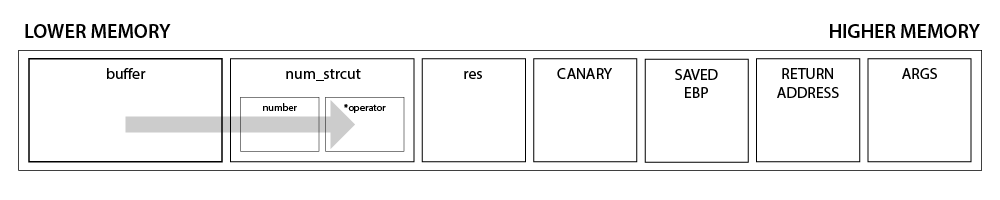
\includegraphics[width=1\columnwidth]{attackStructExpected}
	\captionsource{Résultat attendu de la \og stack frame \fg sur la première attaque}
	{Résultat attendu de la \og stack frame \fg sur la première attaque}
	{Auteur}
	\label{fig:attackStructExpected}
\end{figure}

\subsection{Implémentation}

Le code correspondant au scénario, présenté en \autoref{lst:struct}, comprend: (i) une structure nommée \texttt{Number}, (ii) une fonction \texttt{call()} permettant d'appliquer la fonction pointée par la structure et (iii) une fonction retournant le carré --- très mal optimisé --- de la valeur passée en paramètre. La fonction \texttt{main()} initialise la structure sur la pile ainsi que le \texttt{buffer}, puis copie dans le buffer l'argument \texttt{argv[1]} passé à l'exécution et appelle la fonction \texttt{call()}. De manière théorique il est alors possible, via l'argument \texttt{argv[1]}, de réécrire l'adresse stockée dans la structure.

\begin{listing}
	\cfile{02-main/listings/struct.c}
	\caption{Source du programme lors du premier scénario d'attaque}
	\label{lst:struct}
\end{listing}

Cependant, lorsque l'on inspecte la pile d'exécution, on se rend compte que l'ordre dans lequel les variables sont stockées a été modifié. Le \og buffer \fg est positionné en premier --- vers la gauche ---, ce qui rend impossible son éxploitation. Ce comportement inattendu est le résultat d'une manipulation souhaitée par le compilateur. Afin de se prémunir au mieux contre l'éxploitation des dépassements de tampon, il place les variables de type \mintinline{c}{char*} dans les adresses les plus hautes, juste après le canari. De cette manière, si un dépassement apparaît, il est tout de suite détecté par le canari.

\begin{figure}[H]
	\centering
	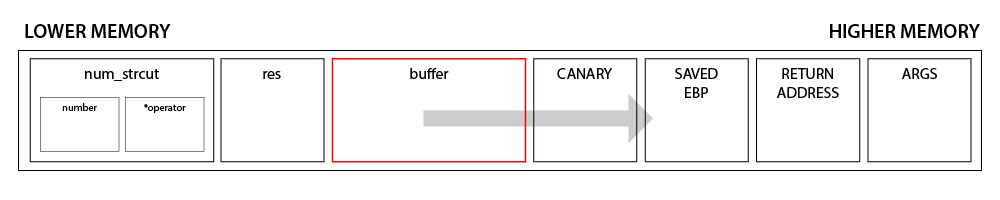
\includegraphics[width=1\columnwidth]{attackStructReel}
	\captionsource{Résultat obtenu de la \og stack frame \fg sur la première attaque}
	{Résultat obtenu de la \og stack frame \fg sur la première attaque}
	{Auteur}
	\label{fig:attackStructReel}
\end{figure}

\subsection{Conclusion}

Cette attaque ne peux pas aboutir et est détectée avec les deux mécanismes de protection. Le but ici est de démontrer les cas de figures où \og \gls{safeStack} \fg permet de se protéger contre des attaques qui ne seraient pas gardée par les \og \gls{stackCookies} \fg, cette attaque est donc abandonée au profit d'une nouvelle approche.


% -----------------------------------------------------------------------------
\section{Bypass du canari}

\subsection{Description théorique de l'attaque}

Le but est toujours d'arriver à lancer une attaque de type \gls{rop}. Pour cela il est
nécessaire d'avoir un point d'entrée afin de démarrer la chaîne. Puisqu'il n'est pas
possible de de réécrire les informations sensibles sur la pile sans passer par le
canari, ce second scénario prévoit un moyen de passer outre la protection en
réécrivant correctement ce dernier.

Le scénario est composé de deux phases distinctes. La première consiste à exploiter
une première faille permettant d'aller lire en mémoire la valeur du canari. La
seconde, une fois le canari obtenu, consiste à démarrer la chaîne de gadgets en
réécrivant la valeur de l'adresse de retour de la fonction, en exploitant une deuxième
faille. Ces deux phases doivent être séquentiellement distinctes et dans l'ordre cité.

Pour récupérer la valeur du canari l'argument \texttt{argv[1]} est utilisé comme
format dans une fonction d'affichage. Il est alors possible d'afficher une suite de
valeurs de pointeurs arbitrairement. Une fois le résultat affiché, l'utilisateur est
solicité afin de rentrer une valeur, valeur qui est ensuite stockée dans le tampon via
une méthode vulnérable aux dépassements.

\begin{figure}[H]
	\centering
	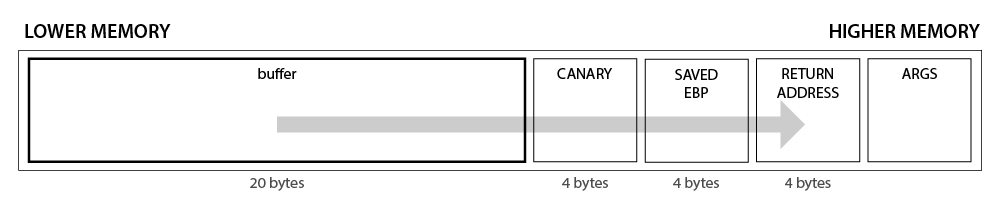
\includegraphics[width=1\columnwidth]{attackCanariLayout}
	\captionsource{Disposition de la pile au sein de la fonction vulnérable}
	{Disposition de la pile au sein de la fonction vulnérable}
	{Auteur}
	\label{fig:attackCanariLayout}
\end{figure}

Le programme imaginé a été conçu de manière à faciliter la mise en place de cette
attaque et ne représente en aucun cas un scénario pertinent au sein d'un environnement
réél. Cependant, les concepts en découlant sont applicable dans tout les cas, ici les
erreurs sont volontairement grossière, mais il est fort probable que des cas
d'attaques similaires, plus complexe à mettre en place, se présentes.

Afin de démontrer la réussite de l'attaque, la chaîne de gadgets doit exécuter deux
fonctions construisant une chaîne de caractères qui est ensuite utilisée comme
paramètre de la fonction \texttt{system()}, au sein d'une troisième fonction. Là
encore, la finalité est prépondérante à la réalité, il faut aussi prendre en compte le
peu de gadgets disponibles au sein d'un programme de si petite taille. La chaîne de
caractères ainsi créée contient la commande \texttt{"echo hacked! > hacked.txt"} afin
de facilement juger la réussite ou l'échec de l'attaque.


\subsection{Implémentation}

La source du programme est plutôt simpliste, la fonction \texttt{main()} appelle la
fonction vulnérable avec l'argument \texttt{argv[1]}. Celui-ci est utilisé directement
comme paramètre de la fonction \texttt{printf()}, un \textit{flush} est ensuite
effectué afin de forcer la sortie dans \textit{stdout}. Le \texttt{buffer} de 20
caractères est initialisé à la ligne 24 et la fonction \texttt{gets()} permet d'écrire
une quantité arbitraire d'octets en mémoire --- jusqu'au caractère
\texttt{\textbackslash n} ou \gls{eof} ---, le contenu du tampon est ensuite réaffiché
de manière à simplifier le débogage. Les deux failles de sécurité se trouve donc aux
lignes 25 et 28.

\begin{listing}
	\cfile{02-main/listings/rop2.c}
	\caption{Source du programme lors du second scénario d'attaque}
	\label{lst:rop2}
\end{listing}

Les fonctions \texttt{add\_bin()} et \texttt{add\_sh()} permettent de construire la
chaîne de caractères exécutée dans la fonction \texttt{system()}. Dans la version
originale de l'attaque ces deux fonctions permettaient d'ouvrir un terminal, d'où leur
nom. Afin de représenter au mieux les concepts de \gls{rop}, des paramètres doivent
être passés aux fonctions. Dans ce cas-ci, ces paramètres n'ont pas d'importance.

\subsection{Éxploitation}

La première étape de l'éxploitation consiste à mettre en place un un script permettant
de gérer le \texttt{stdin} et le \texttt{stdout} du programme de manière à récupérer
la valeur du canari et calculer le \textit{payload} à renvoyer.

Le programme avec les \og \gls{stackCookies} \fg est lancé à la ligne 13 du
\autoref{lst:exploit2} avec comme argument $40 \times$ la valeur \texttt{"\%p"}
permettant de faire un \textit{dump} de la mémoire de la pile. La ligne 19 récupère le
\textit{dump} de mémoire puis recherche l'index où apparaît la valeur
\texttt{0x80486ce}. Cette valeur est l'adresse de la fonction \texttt{main()} qui, au
sein de la fonction \texttt{vulnerable\_function()}, équivaut à l'adresse de retour.
En partant de cet index il est ensuite possible de retrouver la valeur du canari.

\begin{listing}
	\pythonfile{02-main/listings/exploit2.py}
	\caption{Script python instrumentant l'attaque ROP du deuxième scénario sur les \og \gls{stackCookies} \fg}
	\label{lst:exploit2}
\end{listing}

Le \textit{payload} doit permettre d'initialiser la pile d'exécution de manière à
chaîner les gadgets. Pour ce faire, le \texttt{buffer} est rempli avec une valeur
arbitraire, dans ce cas \texttt{"A"}, puis on place la valeur du canari, vient ensuite
une valeur quelconque pour remplacer la valeur sauvegardée de \texttt{\%ebp} et enfin
la chaîne de gadgets.

\begin{listing}
	\textfile{02-main/listings/stack.res}
	\caption{État souhaité de la pile d'exécution après injection du \textit{payload}}
	\label{lst:stackAfterPayload}
\end{listing}

Lorsque l'on test la version \og \gls{stackCookies} \fg avec une entrée trop grande,
le dépassement est bien detecté. La \autoref{lst:stackSmashingDetected} montre le
message qui est affiché avec les diverses informations sur
l'état de la mémoire et de la pile au moment ou l'attaque est détectée.

\begin{listing}
	\textfile{02-main/listings/detected.res}
	\caption{Message obtenu lorsqu'un dépassement de tampon est détecté avec \og \gls{stackCookies} \fg}
	\label{lst:stackSmashingDetected}
\end{listing}

Lorsque l'on exécute le script python le résultat tout autre. Le canari étant de type
\og \textit{random canary} \fg, finissant toujours par \texttt{\textbackslash x00},
l'éxploitation se déroule sans problème. Le canari est trouvé et réécrit correctement
puis la chaîne de gadgets s'exécute comme prévu. Le script affiche la valeur du canari
trouvé et on constate que le fichier \texttt{hacked.txt} qui n'était pas présent est
bien créé.

\begin{listing}
	\textfile{02-main/listings/powned.res}
	\caption{Message obtenu par le script python du second scénario}
	\label{lst:powned}
\end{listing}

C'est au tour de \og \gls{safeStack} \fg de résister à ce scénario d'attaque.
Pour ce faire, vu qu'il n'y a plus de canari, une adaptation du script
python est faite. Ce script est une version simplifiée du précédent, plus besoin de se
soucier du premier résultat revoyé.

Lorsqu'on lance l'exécutable compilé avec \og \gls{safeStack} \fg et que l'on rempli
le tampon avec plus de 20 caractères, on remarque que rien ne se passe. Le mécanisme enlève complétement toutes les possibilités d'éxploitations.

\begin{listing}
	\textfile{02-main/listings/attackSafeStack.res}
	\caption{Rien ne se passe lorsque l'on dépasse la capacité initiale du tampon si le binaire est protégé avec \og \gls{safeStack} \fg}
	\label{lst:attackSafeStack}
\end{listing}

Si on regarde de plus prêt l'état de la pile après injection du \textit{payload}, on
constate que celui-ci, n'étant pas présent dans la même région de mémoire, ne peut
plus altérer les pointeurs et les adresses de la pile régulière.

\begin{listing}
	\textfile{02-main/listings/stackSS.res}
	\caption{État de la pile lors du dépassement de tampon avec \og \gls{safeStack} \fg}
	\label{lst:stackSS}
\end{listing}

Les mécansimes de protéction présent au sein des exécutables sont disponibles en \autoref{chap:mecanismeProtection}. La différence des binaires entre les \og \gls{stackCookies} \fg et \og \gls{safeStack} \fg y est présentée.

\begin{listing}
	\pythonfile{02-main/listings/exploit2-ss.py}
	\caption{Script python instrumentant l'attaque ROP du deuxième scénario sur \og \gls{safeStack} \fg}
	\label{lst:exploit2}
\end{listing}

% -----------------------------------------------------------------------------
\section{Conclusions}

\og Safe stack \fg enlève complétement un des biais utilisé afin de dérouté le flot de
contrôle d'une application. Du moment ou tous les tampons sont déplacés hors de portée
des données sensibles de la pile --- adresses de retour, pointeur de fonctions, etc.
--- il est théoriquement impossible de dérouter le flot de contrôle.

\chapter{Conclusions}
\label{chap:conclusions}

% -----------------------------------------------------------------------------
\section{Les innovations apportées par Levee}

L'innovation majeur présente au sein de \gls{cpi} est l'approche avec laquelle
les chercheurs ont abordés la problématique de protection du flot de contrôle.
Comme montré, il existe déjà des mécanismes tels que SoftBound+CETS,
permettant de se prémunir à 100\% contre les \og control-flow hijack \fg.
Ces mécanismes appliquent les principes des langages \og memory safe \fg sur
l'entièreté du programme, alors que l'approche de \gls{cpi} sélectionne une
partie réduite des pointeurs responsables du flot de contrôle du programme.
Les résultats obtenu, tant en terme de performance qu'en terme d'efficacité,
sont très bons.

Des améliorations telles que HardBound ou Watchdog réduisant le coût en
performance de SoftBound existent. Ces améliorations repose sur des bases
hardware, permettant d'instrumenter la protection de la manière la plus efficace
possible et de soulager la couche software. Pour \gls{levee}, il en va de même,
il est possible d'augmenter les performances en se basant sur des implémentation
hardware tel que, par exemple, Intel MPX (Memory Protection Extensions)
\cite{IntelMPX}, apparu dans l'architecture Skylake, supportée au niveau
du noyau Linux depuis la version 3.19.

\subsection{\og Safe stack \fg}

\og Safe stack \fg se démarque des \og \gls{stackCookies} \fg également par
son approche, au lieu de vouloir protéger seulement les arguements et les adresses
présentes sur la pile d'exécution, les variables accèdées de manière dangereuse
sont déplacées. Les canaris empêchent déjà le démarrage d'une attaque \gls{rop} depuis
la pile, cependant il est possible, sous certaines conditions, de réécrire correctement
le canari et donc de passer outre la protection.

\og Safe stack \fg rend totalement impossible l'exploitation d'un dépassement de
tampon sur la pile par le simple fait que le tampon ne se retrouvera plus sur la pile,
mais dans une zone spéciale présente au sein du segment de \og memory mapping \fg.

% -----------------------------------------------------------------------------
\section{Évaluation des objectifs initiaux}

Les objectifs obligatoires du projet, tel que décrit dans le cahier des charges en
annexe, ont été remplis. Les deux concept \gls{cpi} et \gls{cps} ont été présentés
avec \og \gls{safeStack} \fg. Une description de \gls{llvm} ainsi que l'architecture
de l'implémentation de \og \gls{safeStack} \fg a été rédigée. Un historique des
méthodes de protection ainsi que certaines attaques liées fait office de vue
synoptique des attaques agissant sur le flot de contrôle comme discuté durant
le travail. Deux exemples d'attaque permettant de tester les limites des canaris
ainsi que de \og \gls{safeStack} \fg ont été décrits.

L'objectif optionnel d'analyser les coûts d'un portage de \gls{levee} sur la plateforme
ARM n'a pas été réalisé au moment où ses lignes sont rédigées, bien que la plupart
des éléments nécessaires à cette analyse soit présente dans ce rapport, le temps
a manqué à produire un chapitre ou une section bien documentée concernant les
enjeux à prendre en compte.

\newpage

% -----------------------------------------------------------------------------
\section{Difficultés rencontrées}

La maîtrise du sujet traité a fait défaut au début du travail, une phase importante
de recherche et de compréhension des éléments sur lesquels se basent les
concepts décrits a été nécessaire. C'est aussi pourquoi les sections dédiées aux
récapitulatifs sont aussi fournies pour un rapport de ce type. Aujourd'hui je peux
dire que le sujet en général a bien été parcouru et certains aspects ont été
étudiés plus en profondeur. Les enjeux majeurs et les concepts les plus importants
ont été relayés dans ce rapport avec les explications nécessaires à leur bonne
compréhension.

La mise en place des attaques a été un long chemin parfois difficile. Le chapitre
contient plusieurs attaques documentées afin de représenter la quantité de travail
fournie.

% -----------------------------------------------------------------------------
\section{Sujets de recherche à développer}

On peut distinguer deux parties, \gls{cpi} et \og \gls{safeStack} \fg.
Pour \gls{cpi} les sujets de recherche à développer en premier serait l'intégration
de la technologique Intel MPX, le papier la mentionnait comme étant une technologie
à paraître, maintenant que celle-ci existe il serait intéressant de l'étudier de
plus prêt.

Pour \og \gls{safeStack} \fg, le sujet à développer plus en profondeur pourrait
être sa comparaison avec d'autres moyens permettant de se protéger des dépassements
de tampons.

% Rajout de la description thèorique de CPI proof of correctness


% Appendices
\appendix
\chapter{Configuration du Docker}
\label{chap:dockerConf}

Le docker-compose s'occupe du démarage d'un ou plusieurs container ainsi que de leur interaction avec l'hôte (volumes, ports, etc). Un seul volume partagé est monté au sein du container, sous l'adresse \mintinline{bash}{/shared}. Afin de pouvoir désactiver certaines protection tel que \gls{aslr}, il est nécessaire d'autorisé des privilèges suppérieurs au container (voir ligne 6).

\begin{listing}
	\yamlfile{02-main/listings/docker-compose.yml}
	\caption{Fichier de configuration général utilisé par docker-compose}
	\label{lst:dockerCompose}
\end{listing}

Le contenu d'un fichier \mintinline{bash}{.bash_profile} est copié lors de la phase de contruction du container dans le dossier de l'utilisateur et est rajouté au fichier \mintinline{bash}{.bashrc}, cela permet de rajouter facilement des commandes ou des raccourcis. Actuelement le fichier ne contient pas grand chose mais le méchanisme est en place.

\begin{listing}
	\bashfile{02-main/listings/bashProfile}
	\caption{Fichier bash copier dans le .bashrc de l'utilisateur Debian}
	\label{lst:bashProfile}
\end{listing}

Le fichier principal contenant les instructions de construction de l'image est dispnible au code \ref{lst:dockerfile}.


% -----------------------------------------------------------------------------
% Back matter
% -----------------------------------------------------------------------------
\backmatter

% Bibliography
\cleardoublepage

\printbibliography[title={Références}, heading=bibintoc]

% Glossary
\cleardoublepage
\printglossaries

\end{document}
